\documentclass[12pt]{article}
\usepackage[spanish]{babel}
\usepackage{amsmath}
\usepackage{graphicx}

\usepackage{bigints}

\tolerance=1
\emergencystretch=\maxdimen
\hyphenpenalty=10000
\hbadness=10000

\widowpenalty=10000
\clubpenalty=10000

\usepackage{titlesec}

\setcounter{secnumdepth}{4}

\titleformat{\paragraph}
{\normalfont\normalsize\bfseries}{\theparagraph}{1em}{}
\titlespacing*{\paragraph}
{0pt}{3.25ex plus 1ex minus .2ex}{1.5ex plus .2ex}

\title{Microondas}

\begin{document}

\tableofcontents
\newpage

\section{Introducci\'on a las Microondas}
\subsection{Definici\'on}
La definici\'on del t\'ermino Microondas se puede enfocar b\'asicamente desde dos perspectivas. Una primera, m\'as exacta, que est\'a relacionada con el espectro de frecuencias que abarca, en este caso entre 300 MHz y 300 GHz (en la actualidad esta definici\'on se ha extendido hasta 1 THz). Tambi\'en es habitual encontrar esta definici\'on en t\'erminos de longitudes de onda. Frecuencia, longitud de onda y velocidad de propagaci\'on en un medio homog\'eneo caracterizado por su permitividad el\'ectrica ($\varepsilon$) y magn\'etica ($\mu$) se relacionan seg\'un las f\'ormulas:
$$\lambda = \cfrac{v}{f} \hspace{1cm} v=\cfrac{1}{\sqrt{\mu\varepsilon}} \hspace{1cm} c=\cfrac{1}{\sqrt{\mu_0\varepsilon_0}} \approx 3 \cdot 10^8 \text{m/s} $$

De modo que las microondas quedan comprendidas, en t\'ermimos de $\lambda$, entre 1 m y 1 mm (0,3 mm en el caso de 1 THz). A las se\~nales con longitudes de onda del orden de mil\'imetros se las conoce como ondas milim\'etricas.

\vspace{0.4cm}
La otra definici\'on, menos precisa, es: ``aquella porci\'on del espectro electromagn\'etico en el que las dimensiones de los circuitos son comparables a las longitudes de onda que manejan''. En este sentido, lo que entendemos por teor\'ia de circuitos es un caso especial de la teor\'ia electromagn\'otica descrita mediante las ecuaciones de Maxwell. En Microondas no es v\'alida la aproximaci\'on de elementos discretos o puntuales (concentrados), como en teor\'ia de circuitos. Las componentes de microondas normalmente son elementos distribuidos, donde la fase de una tensi\'on o de una corriente cambia apreciablemente a lo largo del dispositivo, debido a que sus dimensiones son comparables con la longitud de onda. Esta definici\'on tiene en cuenta que el cambio de fase de las componentes de una se\~nal es inversamente proporcional a la longitud de onda:

$$V(t) = a(t) \cos\left(\omega t -\cfrac{2\pi}{\lambda}z\right)$$

por lo que a frecuencias bajas (longitudes de onda grandes), si el tama\~no del circuito es peque\~no, $z_{max}/\lambda <<1$, el cambio de fase es irrelevante. Sin embargo a frecuencias de microondas es un factor fundamental.

\vspace{0.4cm}
En el otro extremo del espectro se encuentra la ingenier\'ia \'optica, donde la longitud de onda es mucho m\'as peque\~na que las dimensiones de los componentes. En este caso las ecuaciones de Maxwell se pueden simplificar mediante la geometr\'ia \'optica. Estas t\'ecnicas se utilizan algunas veces con ondas milim\'etricas y se las conoce como cuasi\'opticas.
\vspace{0.4cm}

En microondas, por tanto, se deber\'a trabajar con las ecuaciones de Maxwell y con sus soluciones. Esto significa que existir\'a en muchos casos una complejidad matem\'atica importante, apareciendo derivadas sobre funciones vectoriales y operaciones con integrales de campos vectoriales, donde estos a su vez dependen de las coordenadas espaciales. Una de las finalidades en microondas ser\'a reducir esta complejidad matem\'atica y encontrar soluciones expresadas en t\'erminos de teor\'ia de circuitos. Generalmente la soluci\'on de teor\'ia de campos presenta una descripci\'on completa del campo electromagn\'etico en cada punto del espacio, resultando m\'as informaci\'on de la que realmente se necesita. Ser\'a preferible poder expresar las soluciones en t\'erminos de teor\'ia de circuitos como potencia, impedancia, tensi\'on, corriente, etc.


\subsection{El Espectro Electromagn\'etico}
Se denomina espectro electromagn\'etico a la distribuci\'on energ\'etica del conjunto de las ondas electromagn\'eticas. Referido a un objeto, se denomina espectro electromagn\'etico o simplemente espectro a la radiaci\'on electromagn\'etica que emite (espectro de emisi\'on) o absorbe (espectro de absorci\'on) una sustancia. Dicha radiaci\'on sirve para identificar la sustancia de manera an\'aloga a una huella dactilar. Los espectros se pueden observar mediante espectroscopios que, adem\'as de permitir observar el espectro, permiten realizar medidas sobre \'este, como la longitud de onda, la frecuencia y la intensidad de la radiaci\'on.
\vspace{0.4cm}

El espectro electromagn\'etico se extiende desde las bajas frecuencias usadas para la radio moderna (extremo de la onda larga) hasta los rayos gamma (extremo de la onda corta), que cubren longitudes de onda de entre miles de kil\'ometros y una fracci\'on del tama\~no de un \'atomo. Se piensa que el l\'imite de la longitud de onda corta est\'a en las cercan\'ias de la longitud de Planck, mientras que el l\'imite de la longitud de onda larga es el tama\~no del universo mismo, aunque en principio el espectro sea infinito y continuo.

\subsubsection{Rango del espectro}
El espectro cubre la energ\'ia de ondas electromagn\'eticas que tienen longitudes de onda diferentes. Las frecuencias de 30 Hz y m\'as bajas pueden ser producidas por ciertas nebulosas estelares y son importantes para su estudio. Se han descubierto frecuencias tan altas como $2.9\cdot 10^{27}$ Hz a partir de fuentes astrof\'isicas.
\vspace{0.4cm}

La energ\'ia electromagn\'etica en una longitud de onda particular λ (en el vac\'io) tiene una frecuencia asociada $f$ y una energ\'ia fot\'onica $E$. As\'i, el espectro electromagn\'etico puede expresarse en t\'erminos de cualquiera de estas tres variables, que est\'an relacionadas mediante ecuaciones
\vspace{0.4cm}

De este modo, las ondas electromagn\'eticas de alta frecuencia tienen una longitud de onda corta y energ\'ia alta, y las ondas de frecuencia baja tienen una longitud de onda larga y energ\'ia baja.
\vspace{0.4cm}

Siempre que las ondas de luz (y otras ondas electromagn\'eticas) se encuentran en un medio (materia), su longitud de onda se reduce. Las longitudes de onda de la radiaci\'on electromagn\'etica, sin importar el medio por el que viajen, son, por lo general, citadas en t\'erminos de longitud de onda en el vac\'io, aunque no siempre se declara expl\'icitamente.
\vspace{0.4cm}

Generalmente, la radiaci\'on electromagn\'etica se clasifica por la longitud de onda: ondas de radio, microondas, infrarrojo y regi\'on visible, que percibimos como luz, rayos ultravioletas, rayos X y rayos gamma.

\vspace{0.4cm}

El comportamiento de la radiaci\'on electromagn\'etica depende de su longitud de onda. Las frecuencias m\'as altas tienen longitudes de onda m\'as cortas, y las frecuencias inferiores tienen longitudes de onda m\'as largas. Cuando la radiaci\'on electromagn\'etica interacciona con \'atomos y mol\'eculas, su comportamiento tambi\'en depende de la cantidad de energ\'ia por cuanto que transporta. La radiaci\'on electromagn\'etica puede dividirse en octavas (como las ondas sonoras).
\vspace{0.4cm}

La espectroscopia puede descubrir una regi\'on mucho m\'as amplia del espectro que el rango visible de 400 nm a 700 nm. Un espectroscopio de laboratorio com\'un puede descubrir longitudes de onda desde 2 nm a 2500 nm. Con este tipo de aparatos puede obtenerse informaci\'on detallada sobre las propiedades f\'isicas de objetos, gases o incluso estrellas. La espectrometr\'ia se usa sobre todo en astrof\'isica. Por ejemplo, muchos \'atomos de hidr\'ogeno emiten ondas de radio que tienen una longitud de onda de 21,12 cm.

\subsubsection{Tipos de radiaci\'on}
Aunque el esquema de clasificaci\'on suele ser preciso, en realidad existe algo de trasposici\'on entre tipos vecinos de energ\'ia electromagn\'etica. Por ejemplo: las ondas de radio a 60 Hz pueden ser recibidas y estudiadas por astr\'onomos, o pueden ser conducidas a lo largo de cables como energ\'ia el\'ectrica. Tambi\'en, algunos rayos gamma de baja energ\'ia realmente tienen una longitud de onda m\'as larga que algunos rayos X de gran energ\'ia. Esto es posible porque ``rayo gamma'' es el nombre que se le da a los fotones generados en la descomposici\'on nuclear u otros procesos nucleares y subnucleares, mientras que los rayos X son generados por transiciones electr\'onicas que implican electrones interiores muy energ\'eticos. Por lo tanto, la diferencia entre rayo gamma y rayo X est\'a relacionada con la fuente de radiaci\'on m\'as que con la longitud de onda de la radiaci\'on. Generalmente, las transiciones nucleares son mucho m\'as energ\'eticas que las transiciones electr\'onicas, as\'i que los rayos gamma suelen ser m\'as energ\'eticos que los rayos X.

\paragraph{Radiofrecuencia}

Las ondas de radio suelen ser utilizadas mediante antenas del tama\~no apropiado (seg\'un el principio de resonancia), con longitudes de onda en los l\'imites de cientos de metros a aproximadamente un mil\'imetro. Se usan para la transmisi\'on de datos, a trav\'es de la modulaci\'on. La televisi\'on, los tel\'efonos m\'oviles, las resonancias magn\'eticas, o las redes inal\'ambricas y de radioaficionados, son algunos usos populares de las ondas de radio.
\vspace{0.4cm}

Las ondas de radio pueden transportar informaci\'on variando la combinaci\'on de amplitud, frecuencia y fase de la onda dentro de una banda de frecuencia. El uso del espectro de radio est\'a regulado por muchos gobiernos mediante la asignaci\'on de frecuencias. Cuando la radiaci\'on electromagn\'etica impacta sobre un conductor, se empareja con \'el y viaja a lo largo del mismo, induciendo una corriente el\'ectrica en la superficie de ese conductor mediante la excitaci\'on de los electrones del material de conducci\'on. Este efecto (el efecto piel) es usado en las antenas. La radiaci\'on electromagn\'etica tambi\'en puede hacer que ciertas mol\'eculas absorban energ\'ia y se calienten, una caracter\'istica que se utiliza en los microondas.

\paragraph{Microondas}
La frecuencia super alta (SHF) y la frecuencia extremadamente alta (EHF) de las microondas son las siguientes en la escala de frecuencia. Las microondas son ondas lo suficientemente cortas como para emplear gu\'ias de ondas met\'alicas tubulares de di\'ametro razonable. La energ\'ia de microondas se produce con tubos klystron y tubos magnetr\'on, y con diodos de estado s\'olido como los dispositivos Gunn e IMPATT. Las microondas son absorbidas por la mol\'eculas que tienen un momento dipolar en l\'iquidos. En un horno microondas, este efecto se usa para calentar la comida. La radiaci\'on de microondas de baja intensidad se utiliza en Wi-Fi.
\vspace{0.4cm}

El horno microondas promedio, cuando est\'a activo, est\'a en un rango cercano y bastante poderoso como para causar interferencia con campos electromagn\'eticos mal protegidos, como los que se encuentran en dispositivos m\'edicos m\'oviles y aparatos electr\'onicos baratos.

\paragraph{Radiaci\'on Infrarroja}
La parte infrarroja del espectro electromagn\'etico cubre el rango desde aproximadamente los 300 GHz (1 mm) hasta los 400 THz (750 nm). Puede ser dividida en tres partes:

\begin{itemize}
	\item Infrarrojo lejano: desde 300 GHz (1 mm) hasta 30 THz (10 μm). La parte inferior de este rango tambi\'en puede llamarse microondas. Esta radiaci\'on es absorbida por los llamados modos rotatorios en las mol\'eculas en fase gaseosa, mediante movimientos moleculares en los l\'iquidos, y mediante fotones en los s\'olidos. El agua en la atm\'osfera de la Tierra absorbe tan fuertemente esta radiaci\'on que confiere a la atm\'osfera efectividad opaca. Sin embargo, hay ciertos rangos de longitudes de onda (``ventanas'') dentro del rango opaco que permiten la transmisi\'on parcial, y pueden ser usados en astronom\'ia.
	\item Infrarrojo medio: desde 30 a 120 THz (10 a 2,5 $\mu$m). Los objetos calientes (radiadores de cuerpo negro) pueden irradiar fuertemente en este rango. Se absorbe por vibraciones moleculares, es decir, cuando los diferentes \'atomos en una mol\'ecula vibran alrededor de sus posiciones de equilibrio.
	\item Infrarrojo cercano: desde 120 a 400 THz (2500 a 750 nm). Los procesos f\'isicos que son relevantes para este rango son similares a los de la luz visible.
\end{itemize}

\paragraph{Radiaci\'on visible (luz)}
La frecuencia por encima del infrarrojo es la de la luz visible. Este es el rango en el que el Sol y las estrellas similares a \'el emiten la mayor parte de su radiaci\'on. No es probablemente una coincidencia que el ojo humano sea sensible a las longitudes de onda que el sol emite con m\'as fuerza. La luz visible (y la luz cercana al infrarrojo) son absorbidas y emitidas por electrones en las mol\'eculas y \'atomos que se mueven desde un nivel de energ\'ia a otro. La luz que vemos con nuestros ojos es realmente una parte muy peque\~na del espectro electromagn\'etico. Un arco iris muestra la parte \'optica (visible) del espectro electromagn\'etico; el infrarrojo (si pudiera verse) estar\'ia localizado justo a continuaci\'on del lado rojo del arco iris, mientras que el ultravioleta estar\'ia tras el violeta.
\vspace{0.4cm}

La radiaci\'on electromagn\'etica con una longitud de onda entre aproximadamente 400 nm y 700 nm es detectado por el ojo humano y percibida como luz visible. A otras longitudes de onda, sobre todo al infrarrojo cercano (m\'as largo de 700 nm) y al ultravioleta (m\'as corto que 400 nm) tambi\'en se les llama luz a veces, sobre todo cuando la visibilidad para los humanos no es relevante.
\vspace{0.4cm}

Si la radiaci\'on que tiene una frecuencia en la regi\'on visible del espectro electromagn\'etico se refleja en un objeto, como por ejemplo un plato hondo de fruta, y luego impacta en nuestros ojos, obtenemos una percepci\'on visual de la escena. El sistema visual de nuestro cerebro procesa la multitud de frecuencias reflejadas en diferentes sombras y matices, y a trav\'es de este fen\'eomeno psicof\'isico que todav\'ia no se entiende completamente, es como percibir\'iamos los objetos.
\vspace{0.4cm}

En la mayor parte de las longitudes de onda, sin embargo, la informaci\'on transportada por la radiaci\'on electromagn\'etica no es directamente descubierta por los sentidos humanos. Las fuentes naturales producen radiaci\'on electromagn\'etica a trav\'es del espectro, y nuestra tecnolog\'ia tambi\'en puede manipular un amplio rango de longitudes de onda. La fibra \'optica transmite luz que, aunque no es adecuada para la visi\'on directa, puede transportar datos que luego son traducidos en sonido o imagen. La codificaci\'on usada en tales datos es similar a lo que se usa con las ondas de radio.
\paragraph{Luz Ultravioleta}
La siguiente frecuencia en el espectro es el ultravioleta (o rayos UV), que es la radiaci\'on cuya longitud de onda es m\'as corta que el extremo violeta del espectro visible.
\vspace{0.4cm}

Al ser muy energ\'etica, la radiaci\'on ultravioleta puede romper enlaces qu\'imicos, haciendo a las mol\'eculas excepcionalmente reactivas o ioniz\'andolas, lo que cambia su comportamiento. Las quemaduras solares, por ejemplo, est\'an causadas por los efectos perjudiciales de la radiaci\'on UV en las c\'elulas de la piel, y pueden causar incluso c\'ancer de piel si la radiaci\'on da\~na las mol\'eculas de ADN complejas en las c\'elulas (la radiaci\'on UV es un mut\'ageno). El Sol emite una gran cantidad de radiaci\'on UV, lo que podr\'ia convertir r\'apidamente la Tierra en un desierto est\'eril si no fuera porque, en su mayor parte, es absorbida por la capa de ozono de la atm\'osfera antes de alcanzar la superficie.
\paragraph{Rayos X}
Despu\'es del ultravioleta vienen los rayos X. Se usan generalmente para ver a trav\'es de algunos objetos, as\'i como para la f\'isica de alta energ\'ia y la astronom\'ia. Las estrellas de neutrones y los discos de acreci\'on alrededor de los agujeros negros emiten rayos X, lo que nos permite estudiarlos.
\paragraph{Rayos gamma}
Despu\'es de los rayos X vienen los rayos gamma. Son los fotones m\'as energ\'eticos, y no se conoce el l\'imite m\'as bajo de su longitud de onda. Son \'utiles a los astr\'onomos en el estudio de objetos o regiones de alta energ\'ia, y son \'utiles para los f\'isicos gracias a su capacidad penetrante y su producci\'on de radiois\'otopos.
\vspace{0.4cm}

No hay ning\'un l\'imite exactamente definido entre las bandas del espectro electromagn\'etico. Algunos tipos de radiaci\'on tienen una mezcla de las propiedades de radiaciones que se encuentran en las dos regiones del espectro. Por ejemplo, la luz roja se parece a la radiaci\'on infrarroja en que puede resonar algunos enlaces qu\'imicos.

\subsection{Propiedades Y Aplicaciones De Las Microondas}
Las microondas presentan algunas propiedades que hacen interesante su utilizaci\'on. Entre \'estas se pueden destacar las siguientes:
\begin{itemize}
	\item La ganancia de una antena es proporcional al tama\~no el\'ectrico de la antena. Para frecuencias muy altas se consiguen, por tanto, antenas m\'as directivas. Por esta raz\'on, para enlaces punto a punto, las microondas presentan un buen compromiso ya que permiten estructuras f\'isicas relativamente peque\~nas para ganancias elevadas (haces estrechos) y no presentan graves problemas de apuntamiento como ocurrir\'ia en el caso de frecuencias \'opticas.
	\item Mayor ancho de banda. En microondas se puede trabajar con anchos de banda relativamente peque\~nos y en cambio tratar con gran cantidad de informaci\'on. Por ejemplo, un ancho de banda de 1\% a 500 MHZ supone 5 MHz (el ancho de banda de un canal de televisi\'on), mientras que a 50 GHz un ancho de banda de 1\% es de 500 MHz (cerca de 100 canales de televisi\'on).
	\item Transparencia de la Ionosfera. Si bien la ionosfera se comporta como una capa reflectora para las frecuencias de onda corta, a las frecuencias de microondas esta capa es transparente, por lo que estas frecuencias de microondas son utilizadas para comunicaciones tierra-sat\'elite. La radioastronom\'ia utiliza tambi\'en esta propiedad para estudiar las estrellas lejanas a trav\'es de sus radiaciones en la banda de microondas.
	\item Transparencia parcial de la atm\'osfera y propagaci\'on en l\'inea recta. A frecuencias de microondas en la atm\'osfera se puede despreciar el fen\'omeno de refracci\'on pudi\'endose considerar propagaci\'on en l\'inea recta. Sin embargo, si bien los distintos componentes atmosf\'ericos (ox\'igeno, nitr\'ogeno, vapor de agua, anh\'idrido carb\'onico) y las part\'iculas en suspensi\'on en la atm\'osfera (gotas de agua, cristales de hielo, polvo, humo, etc.) no afectan a se\~nales por debajo de 10 GHz, s\'i que afectan a se\~nales de microondas por encima de esta frecuencia. Observando la figura 1.3 se distingue una serie de ventanas entre rayas de absorci\'on que permiten comunicaci\'on.
	\item Interacci\'on con la materia. Cuando una onda electromagn\'etica incide sobre una muestra de material, \'esta absorbe energ\'ia de la onda a frecuencias particulares que son las frecuencias de resonancia del material. Esta resonancia observada a frecuencias de microondas depende de la composici\'on molecular de la materia. En particular, el agua absorbe frecuencias de microondas, lo que le confiere b\'asicamente dos propiedades:
		\begin{itemize}
			\item Calentamiento por microondas (Cocci\'on de alimentos, descongelaci\'on, desinfecci\'on, hipertermia, o secado en procesos industriales, entre otros ejemplos).
			\item Detecci\'on y medidas de mezclas contenidas en un material.
		\end{itemize}
	\item Radiaci\'on no ionizante. Las microondas presentan adem\'as la ventaja de no ser ionizante. Significar\'a esto que la energ\'ia de un fot\'on viene dada por $E=h\cdot f$, donde h es la constante de Planck: $h= 4,14\cdot 10^{-15}$eV. Por lo tanto un fot\'on de microondas tiene una energ\'ia comprendida entre $1,2\cdot 10^{-6}$eV y $1,2\cdot 10^{-3}$eV. Esta energ\'ia resulta insuficiente para romper un enlace qu\'imico y por lo tanto no puede extraer un electr\'on y producir la ionizaci\'on. Otras frecuencias mayores s\'i que presentan problemas de ionizaci\'on como son los rayos X o gamma.
	\item Frecuencias de oscilaci\'on estables. Las oscilaciones at\'omicas m\'as estables conocidas hasta ahora, hidr\'ogeno, cesio y rubidio presentan oscilaciones extraordinariamente estables dentro del rango de las microondas. Cuando un electr\'on hace una transici\'on entre dos niveles de energ\'ia se absorbe o se emite un fot\'on, cuya frecuencia es directamente proporcional a la diferencia de energ\'ia entre los dos niveles.
	\item Secci\'on recta radar grande. El \'area de reflexi\'on efectiva (secci\'on recta radar) de un blanco radar es proporcional normalmente al tama\~no el\'ectrico del blanco. Este hecho, junto con la ganancia de las antenas, hacen que a menudo las microondas se utilicen en aplicaciones de radar.
\end{itemize}

\subsection{Evoluci\'on Hist\'orica}
Si bien puede parecer que las microondas sea un campo de investigaci\'on reciente, se deber\'ia situar sus or\'igenes en el siglo pasado, cuando James Clerk Maxwell (1873) formula los conceptos fundamentales del electromagnetismo. A continuaci\'on se enumeran alguno de los hechos m\'as significativos en el desarrollo de las microondas.

\subsubsection{Primeros descubrimientos}
Como cabe esperar, el origen de unas ecuaciones que reciben el nombre de Maxwell no puede ser otro que el propio f\'isico escoc\'es James Clerk Maxwell. Antes que nada conviene ubicarse en el siglo XIX y repasar cuales eran las tendencias de las teor\'ias el\'ectricas y magn\'eticas de aquella \'epoca. Una clasificaci\'on tradicional de todas las teor\'ias existentes en esa \'epoca es la que establece dos tendencias, las de mentalidad electrodin\'amica y las de mentalidad de campo electromagn\'etico. Dentro del primer grupo se encuentran Andr\'e Marie Ampère, Wilhelm Eduard Weber y Hermann Helmholtz, el primero franc\'es y los segundos alemanes. Mientras que el segundo grupo lo integrar\'ian principalmente Michael Faraday, f\'isico ingl\'es, y el mencionado James Clerk Maxwell tambi\'en brit\'anico. El origen de los cient\'ificos permite que a los del primer grupo se le denomine como los continentales y al segundo grupo de las islas brit\'anicas. Para los continentales la sede de los fen\'omenos el\'ectricos son las cargas y las corrientes o cargas en movimiento, mientras que para el segundo grupo lo es todo el espacio, aun el espacio vac\'io.
\vspace{0.4cm}
	
Tal y como se comentaba anteriormente, fue James Clerk Maxwell, quien demostr\'o por investigaciones te\'oricas, que la luz era un fen\'omeno electromagn\'etico y que la energ\'ia electromagn\'etica se propagaba como ondas en el espacio. Por tanto, es a Maxwell a quien corresponde la gloria de ser el primero que demostr\'o cient\'ificamente la existencia de ondas electromagn\'eticas.
\vspace{0.4cm}
	
En este marco otro f\'isico alem\'an, Heinrich Hertz, evoluciona de las ense\~nanzas electrodin\'amicas recibidas entre otros del mismo Hermann von Helmholtz hacia una conversi\'on en las teor\'ias maxwellianas. Fueron bastantes los experimentos que desarroll\'o Hertz y que le fueron conduciendo hacia la teor\'ia de Maxwell, pero sin duda los que m\'as repercusi\'on tuvieron en este camino fueron los que tuvieron lugar durante su \'epoca de profesor en la Universidad de Karlsruhe. All\'i pudo hacer uso de la sala m\'as grande, el aula magna, que utiliz\'o durante \'epocas de vacaciones para montar sus experimentos. Su tama\~no era de 15 m de largo, 14 m de ancho y 6 m de alto, y ten\'ian seis columnas de hierro paralelas a las paredes longitudinales.
\vspace{0.4cm}
	
Haciendo uso de un dipolo resonante formado por dos varillas terminadas en cada uno de sus extremos por grandes esferas conductoras y esferas conductoras peque\~nas en los otros extremos, y mediante un sistema de excitaci\'on constante, se hac\'ia resonar aquella estructura a una frecuencia de unos 60 MHz.
\vspace{0.4cm}
	
En el otro extremo de la sala ten\'ia ubicada una espira rectangular resonante a la misma frecuencia que ten\'ia insertada un chispero, elemento formado por dos electrodos muy pr\'oximos que hac\'ian saltar chispas cuando se le aplicaba una diferencia de potencial. Para poder ver estas chispas necesitaba oscurecer la sala dada su baja intensidad. Con este sistema de medida midi\'o la velocidad de propagaci\'on de las ondas radiadas mediante la distancia entre los nulos de la onda estacionaria que aparec\'ia al colocar una pared conductora en el extremo contrario de la antena transmisora.
	
\subsubsection{El desarrollo de la gu\'ia de onda}
Hertz nunca desestim\'o la posibilidad de propagar ondas electromagn\'eticas dentro de un tubo hueco de metal. O. Heaviside tambi\'en consider\'o esta posibilidad, desech\'andola arguyendo que era necesario la existencia de dos conductores para la transferencia de energ\'ia electromagn\'etica. En aquellos momentos s\'olo se contemplaba como soluci\'on los modos transversales electromagn\'eticos.
\vspace{0.4cm}
	
En 1897 Lord Rayleigh demostr\'o matem\'aticamente que la propagaci\'on de ondas en gu\'ias era posible tanto para secci\'on circular como para rectangular.
\vspace{0.4cm}

Aunque no se hicieron verificaciones experimentales de la teor\'ia de Rayleigh, en 1894 Sir Oliver Lodge observ\'o el car\'acter direccional de la se\~nal radiada obtenida con un generador de chispa rodeado con un tubo met\'alico. Este efecto se consider\'o como una curiosidad de laboratorio y no pas\'o de ah\'i.
\vspace{0.4cm}

No fue hasta 1936 cuando la gu\'ia de ondas fue redescubierta de forma independiente por dos hombres: George C. Soutworth y Wilner L. Barrow. Estos experimentos se realizaron con ca\~ner\'ias met\'alicas para conducci\'on de agua.
\subsubsection{Desarrollo del radar}
El gran avance de las microondas se debi\'o sin duda al desarrollo del radar en la segunda guerra mundial. De hecho al magnetr\'on se le conoc\'ia como la v\'alvula que gan\'o la guerra. Al final de la guerra, parte de la informaci\'on pas\'o a ser no clasificada, public\'andose por el Massachusetts Institute of Technology, constituyendo el primer cuerpo de doctrina de las microondas.
\subsubsection{Desarrollo de los tubos de microondas}
Los primeros generadores de microondas fueron los tubos de vac\'io. Entre ellos destacan el ya mencionado magnetr\'on y el klystron que fue inventado en 1937 por los hermanos Varian. Posteriormente se desarrollaron el B.W.O (Backward Wave Oscillator) y el tubo de ondas progresivas TWT (Travelling Wave Tube).
\subsubsection{Dispositivos de ferrita}
El primer dispositivo lineal, pasivo no rec\'iproco apareci\'o en 1956, un girador inventado por C. Lester Hogan. Los numerosos aisladores y circuladotes desarrollados desde entonces son fundamentalmente utilizados como protecci\'on, desacoplo y control. En todos o casi todos los equipos de microondas pueden verse dispositivos de este tipo en la actualidad.

\subsubsection{Comunicaciones por sat\'elite}
En 1962 fue lanzado el Telstar, el primer sat\'elite de comunicaciones situado en una \'orbita baja. Tres a\~nos m\'as tarde, en 1965 se sit\'ua en \'orbita geoestacionaria el sat\'elite Early Bird. Desde entonces sucesivas generaciones de sat\'elites han jugado un papel importante en las comunicaciones, sobre todo en enlaces internacionales.

\subsubsection{Dispositivos de estado s\'olido}Los dispositivos activos semiconductores aparecen en el mercado sobre los a\~nos 60, reemplazando a los tubos como fuentes de microondas para potencias medias y bajas. El primer dispositivo desarrollado de este tipo fue el diodo Gunn, basado en un fen\'omeno f\'isico descubierto por J.B. Gunn en 1962. A finales de los a\~nos 70 se empezaron a utilizar los primeros transistores de microondas tanto bipolares como MESFET’s. Esto se debi\'o fundamentalmente a la mejora en la tecnolog\'ia fotolitogr\'afica que permiti\'o metalizaciones muy estrechas. Este mismo avance permiti\'o la sustituci\'on parcial de las gu\'ias de onda por circuitos impresos de microondas, tales como la l\'inea microstrip, la l\'inea slot-line o la l\'inea coplanar. En nuestros d\'ias se est\'an desarrollando circuitos que integran l\'ineas, dispositivos activos y otros componentes en un solo substrato semiconductor, formando lo que se conoce por circuito monol\'itico integrado de microondas (MMIC: Monolithic Microwave Integrated Circuit). Esta tecnolog\'ia permitir\'a abaratar la circuiter\'ia de microondas y reducir el tama\~no de sus sistemas.
\vspace{0.4cm}
	
Es importante notar que este tipo de tecnolog\'ia requiere un dise\~no m\'as exacto y ajustado que los circuitos compuestos por elementos discretos, en los que era posible su ajuste a posteriori. Es por ello imprescindible para el correcto desarrollo de esta tecnolog\'ia el disponer de t\'ecnicas de simulaci\'on fiables (CAD: Computer Aided Design).

\subsection{Problemas Asociados a Las Frecuencias de Microondas}
Sin duda podemos decir que el campo m\'as valioso de aplicaci\'on de las microondas es el de las comunicaciones, desde las que pudi\'eramos denominar privadas, pasando por las continentales e intercontinentales, hasta llegar a las extraterrestres. En este terreno, las microondas act\'uan generalmente como portadoras de informaci\'on, mediante una modulaci\'on o codificaci\'on apropiada. En los sistemas de radar, cabe citar desde los empleados en armamento y navegaci\'on, hasta los utilizados en sistemas de alarma; estos \'ultimos sistemas suelen tambi\'en basarse en efecto DOPPLER o en cambios que sufre la raz\'on de onda estacionaria (SWR) de una antena, pudiendo incluso reconocerse la naturaleza del elemento de alarma. Sistema autom\'atico de puertas, medida de velocidad de veh\'iculos, etc
\vspace{0.4cm}
	
Otro gran campo de aplicaci\'on es el que se pudiera denominar cient\'ifico, como el estudio de materiales, medicina y biolog\'ia, sin embargo, un crecimiento incontrolado de la utilizaci\'on de las microondas, puede dar lugar a problemas no solo de congesti\'on del espectro, interferencias, etc., sino tambi\'en de salud humana; este \'ultimo aspecto no est\'a lo suficientemente estudiado, como se deduce del hecho de que los \'indices de peligrosidad sean marcadamente diferentes de unos pa\'ises a otros.
\vspace{0.4cm}
	
Centr\'andonos en la aplicaci\'on de las microondas a las comunicaciones, podemos decir que un enlace v\'ia microondas consiste en tres componentes fundamentales: El Transmisor, El receptor y El Canal A\'ereo. El Transmisor es el responsable de modular una se\~nal digital a la frecuencia utilizada para transmitir y posee una antena con una corta y flexible gu\'ia de onda, El Canal A\'ereo representa un camino abierto entre el transmisor y el receptor, y como es de esperar el receptor es el encargado de capturar la se\~nal transmitida y llevarla de nuevo a se\~nal digital. El factor limitante de la propagaci\'on de la se\~nal en enlaces microondas es la distancia que se debe cubrir entre el transmisor y el receptor.
\vspace{0.4cm}
	
A estas frecuencias el camino entre el transmisor y el receptor ha de ser directo, ya que las microondas son muy sensibles a la presencia de obst\'aculos, ello implica que las antenas se tengan que instalar en torres. Otro problema muy importante asociado a las microondas son las condiciones atmosf\'ericas, ya que pueden ocasionar desvanecimientos intensos y desviaciones del haz, lo que implica utilizar sistemas de diversidad y equipos auxiliares lo que supone un importante problema en dise\~no. Las interferencias a estas frecuencias tambi\'en pueden llegar a ser inconveniente, ya que la proliferaci\'on de estos sistemas puede dar lugar a solapamiento entre las se\~nales. Por \'ultimo cabe destacar que las microondas son susceptibles a un fen\'omeno denominado Desvanecimiento Multicamino (Multipath Fading) que se produce cuando una se\~nal de radio se divide al ser transmitida en varias se\~nales, y cada una de estas se\~nales viaja a trav\'es de un camino distinto antes de llegar al receptor lo que puede causar una profunda disminuci\'on el la potencia de la se\~nal recibida.


\section{La Gu\'ia de Onda Rectangular y Circular. El Cable Coaxial}
\subsection{La gu\'ia de onda como l\'inea de transmisi\'on}

La gu\'ia de onda es una l\'inea de transmisi\'on (secci\'on constante a lo largo, simetr\'ia cil\'indrica), formada por un diel\'ectrico (aire, por ejemplo) rodeado por un conductor, en forma rectangular o circular. Sus caracter\'isticas de inter\'es ser\'an:
\begin{itemize}
	\item Configuraci\'on espacial de los campos electromagn\'eticos (modos de propagaci\'on).
	\item Frecuencia de Corte: frecuencia m\'inima para la existencia de propagaci\'on de onda dentro de la gu\'ia.
	\item Longitud de onda de los modos.
	\item Constantes de propagaci\'on y atenuaci\'on.
	\item Impedancia de modo.
\end{itemize}

\subsection{Ec. de Maxwell en la gu\'ia de onda (Modos TE, TM, y TEM)}

Para conocer la distribuci\'on de campos E y H, las ecuaciones de Maxwell nos permiten emplear la densidad de corriente y carga ($\vec{J}$ y $\rho$), as\'i como las condiciones de contorno.

Por simplicidad, suponemos la no existencia de fuentes de corriente ni cargas. Esto particulariza las ec. de Maxwell como:

$$
\begin{array}{ll}
	\nabla \vec{D} = 0 & \nabla \times \vec{E} = - \cfrac{\partial \vec{B}}{\partial t}\\
	\\
	\nabla \vec{B} = 0 & \nabla \times \vec{H} = - \cfrac{\partial \vec{B}}{\partial t}
\end{array}
\hspace{0.5cm}
\begin{array}{ll}
	D = \varepsilon E    & \varepsilon = \varepsilon_o \varepsilon_r \\
	B = \mu H            & \mu = \mu_o \mu_r \\
	\\
	\varepsilon_o = 8,85 & \cdot 10^{-12} \text{F/m}\\
	\mu_o = 4\pi         & \cdot 10^{-7} \text{F/m}
\end{array}
$$

Asumimos un r\'egimen sinusoidal permanente, de forma que la variaci\'on temporal de los campos ser\'a de la forma $e^{jwt}$ (obviamos la demostraci\'on de que los campos electromagn\'eticos son ondas), por lo que los campos producen un sistema de ecuaciones diferenciales de segundo orden.
$$
\begin{array}{l@{}l}
	\nabla^2\vec{E} + k^2\vec{E} &= 0 \\
	\nabla^2\vec{H} + k^2\vec{H} &= 0
\end{array}
\hspace{1cm}
k = \cfrac{2\pi}{\lambda}
$$

Para resolverlos, asumimos que podemos descomponer los campos el\'ectrico y magn\'etico en sus componentes\footnote{La dependencia de $\tau_1$ y $\tau_2$ se refiere a una funci\'on dependiente de las componentes transversales a $z$ en coordenadas cartesianas o cil\'indricas ($x,y$ \'o $\rho, \varphi$).} axial ($\vec{E}_z = E_z \cdot \hat{z}$ y $\vec{H}_z = H_z \cdot \hat{z}$) y transversal ($ \vec{E}_t$ y $ \vec{H}_t $):

$$\vec{E} = [\vec{E_t}(\tau_1, \tau_2) + E_t(\tau_1, \tau_2)\hat{z}]f(z)$$
$$\vec{H} = [\vec{H_t}(\tau_1, \tau_2) + H_t(\tau_1, \tau_2)\hat{z}]f(z)$$

Donde $f(z) = e^{-\gamma z}$ representa la periodicidad espacial de los campos. De esta forma, obtenemos el sistema de 4 ecuaciones:
$$\nabla^2 _t \cdot E_z + (k^2 + \gamma^2)E_z = 0$$
$$\nabla^2 _t \cdot \vec{E_t} + (k^2 + \gamma^2)\vec{E_t} = 0$$
$$\nabla^2 _t \cdot H_z + (k^2 + \gamma^2)E_z = 0$$
$$\nabla^2 _t \cdot \vec{H_t} + (k^2 + \gamma^2)\vec{H_t} = 0$$

Las ecuaciones 1 y 3 son sobre campos escalares, y resolviendo s\'olo \'estas podemos calcular los campos axiales, y,  a partir de \'estos, los transversales, seg\'un las f\'ormulas:
$$\vec{E_t}= \cfrac{1}{k^2 + \gamma^2}(-j\omega\mu\nabla_t \times H_z \cdot \hat{z} -\gamma \nabla_t E_z)$$
$$\vec{H_t}= \cfrac{1}{k^2 + \gamma^2}(-j\omega\mu\nabla_t \times E_z \cdot \hat{z} -\gamma \nabla_t H_z)$$


\subsection{M\'etodo de an\'alisis de gu\'ias de onda}

Resolvemos la ecuaci\'on de Helmholtz (1 o 3), para $E_z$ o $H_z$, asumiendo que conocemos su dependencia de z.
A fin de cuentas, lo que haremos ser\'a aplicar las condiciones de contorno para obtener las constantes que caracterizan la soluci\'on, que es siempre ``la misma''.


Las infinitas soluciones a las ecuaciones de onda se agrupan en 3 conjuntos disjuntos: 
\begin{itemize}
	\item TE (Transversal El\'ectrico): El campo el\'ectrico tiene \'unicamente componente transversal ($E_z = 0$), pero s\'i componente axial magn\'etica ($H_z \neq 0$)
	\item TM (Transversal Magn\'etico): El campo magn\'etico tiene \'unicamente componente transversal ($H_z = 0$), pero s\'i componente axial el\'ectrico ($E_z \neq 0$)
	\item TEM (Transversal Electromagn\'etico): Los campos el\'ectrico y  magn\'etico tienen \'unicamente componente transversal ($E_z = 0$ y $H_z = 0$)
\end{itemize}


Una l\'inea admite la propagaci\'on de modos TEM si contiene al menos 2 componenntes no cortocircuitados a distinto potencial.

La constante de propagaci\'on $\gamma$ se define como $\gamma = \pm jk\sqrt{\mu\varepsilon}$.

\subsubsection{Modos TEM}

Partiendo de $E_z = H_z = 0$, los campos que buscamos son:

$$\vec{E} = \vec{E_t}(\tau_1,\tau_2) e^{j\omega t}$$
$$\vec{H} = \vec{H_t}(\tau_1,\tau_2) e^{j\omega t}$$

Aplicando las Ecuaciones de Maxwell, obtenemos: 

$$
\begin{array}{l}
    \nabla_t \times \vec{E_t} = 0 \\
    \nabla_t \times \vec{H_t} = 0
\end{array}
\rightarrow
\begin{array}{l}
        \nabla_t \vec{E_t} = 0 \\
        \nabla_t \vec{H_t} = 0 \end{array}
\rightarrow
\begin{array}{lr}
        \nabla_z \times \vec{E_t} = & -j\omega\mu\vec{H}_t \\
        \nabla_z \times \vec{H_t} = & j\omega\vec{E}_t \end{array}$$
        
Puesto que el campo ele\'ectrico se puede obtener a partir de la funci\'on potencial $\phi(\tau_1, \tau_2)$, podemos reescribir la primera ecuaci\'on como:

$$\nabla^2_n \phi = 0$$

Resolviendo esta ecuaci\'on, obtenemos el campo $\phi$, y calculamos $\vec{E}$ como $\vec{E}_t = -\nabla_t \phi(\tau_1, \tau_2)$. El campo magn\'etico se obtiene despejando $\vec{H}_t$ como sigue:

$$\vec{H}_t = \cfrac{\gamma}{j\omega\mu}(\Hat{z} \times \vec{E}_t) e^{-\gamma z} = \cfrac{1}{\eta}(\Hat{z} \times \vec{E}_t) e^{-\gamma z}$$

Donde $\eta$ denota la impedancia del medio: $120\pi$ Ohmios en aire o vac\'io.

\vspace{0.5 cm}

El n\'umero de onda de corte de los modos TEM se define como:

$$k_c = k^2 + \gamma^2 = k^2 + (\pm jk^2) = k^2 - k^2 = 0$$

Esto quiere decir que los modos TEM se propagan a frecuencias de est\'atica, sin una frecuencia m\'inima.

\subsubsection{Modos TE}

Los modos TE se caracterizan por $E_z = 0$, por lo que los campos en la gu\'ia se calculan como:

$$\vec{E} = \vec{E_t}(\tau_1,\tau_2) e^{-\gamma z}
\hspace{7mm}
\vec{H} = \vec{H_t}(\tau_1,\tau_2) e^{-\gamma z} + H_z(\tau_1,\tau_2) e^{-\gamma z}\hat{z}$$

Para ello, partimos de la ecuaci\'on:

$$\nabla^2 _n H_z + k_c^2 H_z = 0 \hspace{1cm} k_c^2 = k^2 - \beta^2 \neq 0, H_z \neq 0$$

Aplicando las condiciones de contorno, obtenemos la soluci\'on gen\'erica de $H_{zn}$ (donde $n$ denota el \'indice del modo). A partir de $H_{zn}$, calculamos:

$$\vec{H}_{tn} = \cfrac{-\gamma_n}{k^2_cn}\nabla_t H_{zn}
\hspace{7mm}
\vec{E}_{tn} = \cfrac{j\omega\mu}{k^2_{cn}} \nabla_t \times (H_{zn}\hat{z}) = -\cfrac{j\omega\mu}{\gamma_n}\hat{z} \times \vec{H}_{tn}$$

Cada modo presenta una impedancia caracter\'istica distinta, que se calcula como:

$$z_{TEn} = \cfrac{\hat{z} \times \vec{E}_{tn}}{\vec{H}_{tn}} = \cfrac{\vec{E}_{tn}}{\vec{H}_{tn} \times \hat{z}} = \cfrac{j\omega\mu}{\gamma_n}$$

La frecuencia de corte del modo $n$ se define como:

$$f_{cn} = \cfrac{k_{cn}}{2\pi\sqrt{\mu\varepsilon}}$$

\paragraph{Pared El\'ectrica}

Una condici\'on de contorno que encontraremos habitualmente en las gu\'ias de onda es la de pared el\'ectrica. Se da cuando la gu\'ia se compone de paredes conductoras perfectas ($\sigma = \infty$). Las ecuaciones de Maxwell implican que la componente tangencial de campo el\'ectrico a lo largo del contorno de la gu\'ia ha de ser 0; expresando este requisito en t\'erminos de campo magn\'atico, obtenemos:

$$E_z\big|_{\text{contorno}} = \cfrac{\partial H_z}{\partial n}\bigg|_{\text{contorno}} = 0$$

Donde $n$ es la direcci\'on normal al contorno considerado (si, por ejemplo, consideramos un contorno seg\'un la direcci\'on de $y$, nuestra direcci\'on normal ser\'a $x$).

\subsubsection{Modos TM}

Los modos TM se caracterizan por presentar $H_z = 0$, por lo que tenemos que hallar los campos de la forma:

$$\vec{E} = \vec{E_t}(\tau_1,\tau_2) e^{-\gamma z} + E_z(\tau_1,\tau_2) e^{-\gamma z}\hat{z}
\hspace{7mm}
\vec{H} = \vec{H_t}(\tau_1,\tau_2) e^{-\gamma z}$$

Partiendo de la ecuaci\'on:

$$\nabla^2 _n E_z + k_c^2E_z = 0 \hspace{1cm} k_c^2 = k^2 - \beta^2 \neq 0, E_z \neq 0$$

Aplicamos las condiciones de contorno para hallar $E_{zn}$, y lo usamos para calcular:
$$\vec{E}_{tn} = -\cfrac{\gamma_n}{k^2_{cn}}\nabla_t E_z
\hspace{7mm}
\vec{H}_{tn} = \cfrac{j\omega\varepsilon}{k^2_{cn}}\nabla_t \times (E_z \hat{z}) = -\cfrac{j\omega\varepsilon}{k^2_{cn}}\hat{z}\times\nabla_t E_z$$



La frecuencia de corte del modo $n$ se define como:
$$f_{cn} = \cfrac{k_{cn}}{2\pi\sqrt{\mu\varepsilon}}$$

Cada modo presenta una impedancia caracter\'istica distinta, que se calcula como:
$$z_{TMn} = \cfrac{\hat{z} \times \vec{E}_{tn}}{\vec{H}_{tn}} = \cfrac{\vec{E}_{tn}}{\vec{H}_{tn} \times \hat{z}} = \cfrac{\gamma_n}{j\omega\varepsilon}$$

\subsection{La Gu\'ia de Onda Rectangular}

La gu\'ia de onda rectangular se compone de un diel\'ectrico perfecto (no habr\'a p\'erdidas) rodeado por un conductor perfecto ($\sigma = \infty$) que, en secci\'on, forma un rect\'angulo de base $a$ y altura $b$, tal que $a>b$. La direcci\'on de propagaci\'on ser\'a, como de costumbre, $z$.
\begin{center}
	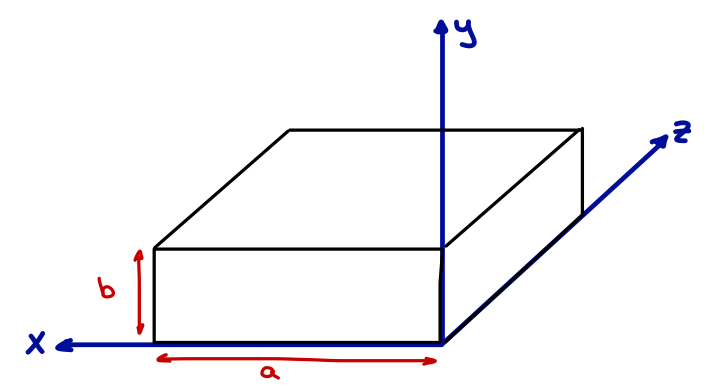
\includegraphics[width=8cm]{img/Guia_de_onda_rectangular.jpg}
\end{center}

Para el an\'alisis de esta gu\'ia, partimos de la ecuaci\'on de onda unidimensional (Donde $A$ representa a $E$ \'o a $H$):
$$\nabla^2 _t A_z + (k^2 + \gamma^2)A_z = 0$$

Y descomponemos la funci\'on $A_z$ en un producto de funciones de una \'unica variable: $A_z(\tau_1, \tau_2) = X(\tau_1) \cdot Y(\tau_2)$. En coordenadas cartesianas, resulta:
$$A_z = [A_1 \cos(k_xx) + B_1\sen(k_xx)][C_1\cos(k_yy) + D_1\sen(k_yy)]$$

Donde $A_1$, $B_1$, $C_1$ y $D_1$ ser\'an constantes que se particularizar\'an seg\'un el campo que calculemos y las condiciones de contorno que queramos satisfacer.

\subsubsection{Modos TE en la Gu\'ia de Onda Rectangular}

Partiendo de que $E_z = 0$, nuestro objetivo es definir $H_z$ con la expresi\'on del apartado anterior:
$$H_z = [A_1 \cos(k_xx) + B_1\sen(k_xx)][C_1\cos(k_yy) + D_1\sen(k_yy)]$$

Despu\'es, procedemos a aplicar las condiciones de pared el\'ectrica para los 4 contornos: $x=0$, $x=a$, $y=0$ e $y=b$, a fin de caracterizar $A_1$, $B_1$, $C_1$ y $D_1$.

\begin{itemize}
	\item $x=0$, $\hat{n} = \hat{x} \rightarrow \cfrac{\partial H_z}{\partial x}\bigg|_{x=0} = 0$
$$[-A_1 k_x \sen(k_xx) + B_1 k_x \cos(k_xx)]\cdot[C_1\cos(k_yy) + D_1\sen(k_yy)]\big|_{x=0} =0$$
$$[-A_1 k_x \sen(0) + B_1 k_x \cos(0)]\cdot[C_1\cos(k_yy) + D_1\sen(k_yy)]=0$$
$$B_1 k_x\cdot[C_1\cos(k_yy) + D_1\sen(k_yy)]=0$$

Como el segundo factor depende de $y$, que var\'ia a lo largo de este contorno, s\'olo podemos manipular el primero.

$$B_1 k_x = 0, k_x \neq 0 \hspace{0.3cm}\rightarrow \hspace{0.3cm} B_1 = 0$$


	\item $x=a$, $\hat{n} = \hat{x} \rightarrow \cfrac{\partial H_z}{\partial x}\bigg|_{x=a} = 0$
$$-A_1 k_x \sen(k_xx)[C_1\cos(k_yy) + D_1\sen(k_yy)]\big|_{x=a} =0$$
$$-A_1 k_x \sen(k_xa)[C_1\cos(k_yy) + D_1\sen(k_yy)] =0$$

Como el segundo factor depende de $y$, que var\'ia a lo largo de este contorno, s\'olo podemos manipular el primero.
$$-A_1 k_x \sen(k_xa) =0$$

Puesto que $k_x \neq 0$ y anular $A_1$ supondr\'ia que no existe campo, tenemos que forzar $\sen(k_xa) =0$, quedando:
$$k_xa = m\pi \hspace{0.3cm}\rightarrow \hspace{0.3cm} k_x=\cfrac{m\pi}{a}\hspace{7mm} m \in [0,1,2...]$$
	\item $y=0$, $\hat{n} = \hat{y} \rightarrow \cfrac{\partial H_z}{\partial y}\bigg|_{y=0} = 0$
$$A_1 \cos\left(\cfrac{m\pi}{a}x\right)\cdot[-C_1k_y\sen(k_yy) + D_1k_y\cos(k_yy)]\big|_{y=0} =0$$
$$A_1 \cos\left(\cfrac{m\pi}{a}x\right)\cdot[-C_1k_y\sen(0) + D_1k_y\cos(0)] =0$$
$$A_1 \cos\left(\cfrac{m\pi}{a}x\right)\cdot D_1k_y =0$$

Ingorando el primer factor, que depende de $x$, y teniendo en cuenta que $k_y \neq 0$, tenemos:
$$D_1=0$$
	\item $y=b$, $\hat{n} = \hat{y} \rightarrow \cfrac{\partial H_z}{\partial y}\bigg|_{y=b} = 0$
$$A_1 \cos\left(\cfrac{m\pi}{a}x\right)\cdot-C_1k_y\sen(k_yy)\big|_{y=b} = 0$$
$$A_1 \cos\left(\cfrac{m\pi}{a}x\right)\cdot C_1k_y\sen(k_yb) = 0$$
	
	Ignorando la parte dependiente de $x$:
$$C_1k_y\sen(k_yb) = 0$$
	Como anular $C_1$ eliminar\'ia el campo y $k_y \neq 0$, forzamos $\sen(k_yb) = 0$:
$$k_yb = n\pi \hspace{0.3cm}\rightarrow \hspace{0.3cm} k_y=\cfrac{n\pi}{b}\hspace{7mm} n \in [0,1,2...]$$

\end{itemize}

Agrupamos $A_1$ y $C_1$ como $A$, la amplitud m\'axima, y la f\'ormula del campo queda:
$$H_z = A \cos\left(\cfrac{m\pi}{a}x\right) \cos\left(\cfrac{n\pi}{b}y\right)$$

Con este resultado podemos calcular $H_t$:

$$\vec{H}_t = - \cfrac{\gamma}{k^2_c} \nabla_t H_z \rightarrow \left\{ \begin{array}{l}
        H_x = \cfrac{\gamma}{k^2_c} \cfrac{m\pi}{a} A \sen \left(\cfrac{m\pi}{a}x\right)\cos\left(\cfrac{n\pi}{b}y\right)\\
        H_y = \cfrac{\gamma}{k^2_c} \cfrac{n\pi}{b} A \cos \left(\cfrac{m\pi}{a}x\right)\sen\left(\cfrac{n\pi}{b}y\right)\\
    \end{array}\right.
$$
Y $\vec{E}_t$:

$$\vec{E}_{t} = -\cfrac{j\omega\mu}{\gamma}\hat{z} \times \vec{H}_{t} = -\cfrac{j\omega\mu}{\gamma}
		\Bigg|
	\begin{array}{lll}
		\hat{x} & \hat{y} & \hat{z}\\
		0 & 0 & 1\\
		H_x & H_y & 0
	\end{array}
	\Bigg|
$$

$$E_y = -\cfrac{j\omega\mu}{\gamma} H_x \hspace{1cm} E_x = \cfrac{j\omega\mu}{\gamma} H_y$$

La impedancia caracter\'istica del modo y el n\'umero de onda de corte se calculan como:

$$ z_{TE} = \cfrac{\mu}{\sqrt{1-\cfrac{k^2}{k^2_c}}}\hspace{1cm} k_c = \sqrt{\left(\cfrac{m\pi}{a}\right)^2 + \left(\cfrac{n\pi}{b}\right)^2}$$

\subsubsection{Modos TM en la Gu\'ia de Onda Rectangular}

Puesto que $H_z = 0$, buscamos calcular:
$$E_z = [A_1 \cos(k_xx) + B_1\sen(k_xx)][C_1\cos(k_yy) + D_1\sen(k_yy)]$$

Para ello, aplicamos las condiciones de contorno:
\begin{itemize}
	\item $x=0 \rightarrow E_z\big|_{x=0} = 0$
	$$[A_1 \cos(k_xx) + B_1\sen(k_xx)][C_1\cos(k_yy) + D_1\sen(k_yy)]\big|_{x=0} = 0$$
	$$[A_1 \cos(0) + B_1\sen(0)][C_1\cos(k_yy) + D_1\sen(k_yy)] = 0$$
	$$A_1[C_1\cos(k_yy) + D_1\sen(k_yy)] = 0$$
	
	Ignorando la parte que depende de $y$:
	$$A_1 = 0$$
	
	\item $x=a \rightarrow E_z\big|_{x=a} = 0$
	$$B_1\sen(k_xx)[C_1\cos(k_yy) + D_1\sen(k_yy)]\big|_{x=a} = 0$$
	$$B_1\sen(k_xa)[C_1\cos(k_yy) + D_1\sen(k_yy)] = 0$$
	
	Ignorando la parte que depende de $y$:
	$$B_1\sen(k_xa) = 0$$
	
	Como anular $B_1$ eliminar\'ia el campo, suponemos que $\sen(k_xa) = 0$:
	
	$$k_xa = m\pi \hspace{0.3cm}\rightarrow \hspace{0.3cm} k_x = \cfrac{m\pi}{a} \hspace{7mm} m \in [0,1,2...]$$
	\item $y=0 \rightarrow E_z\big|_{y=0} = 0$
	$$B_1\sen\left(\cfrac{m\pi}{a}x\right)[C_1\cos(k_yy) + D_1\sen(k_yy)]\big|_{y=0} = 0$$
	$$B_1\sen\left(\cfrac{m\pi}{a}x\right)[C_1\cos(0) + D_1\sen(0)] = 0$$

	Ignorando la parte que depende de $x$:
	$$C_1 = 0$$
	
	\item $y=b \rightarrow E_z\big|_{y=b} = 0$
	$$B_1\sen\left(\cfrac{m\pi}{a}x\right)D_1\sen(k_yy)\big|_{y=b} = 0$$
	$$B_1\sen\left(\cfrac{m\pi}{a}x\right)D_1\sen(k_yb)= 0$$

	Ignorando la parte que depende de $x$:
	$$D_1\sen(k_yb)= 0$$
	
	Como no podemos anular $D_1$ sin eliminar el campo:
	$$\sen(k_yb)= 0 \hspace{0.3cm}\rightarrow \hspace{0.3cm} k_yb = n\pi \hspace{0.3cm}\rightarrow \hspace{0.3cm} k_y = \cfrac{n\pi}{b} \hspace{7mm} n \in [0,1,2...]$$
\end{itemize}

Finalmente, llamando $A$ al producto de $B_1$ y $D_1$, la expresi\'on del campo queda:
$$E_z = A\sen\left(\cfrac{m\pi}{a}x\right)\sen\left(\cfrac{n\pi}{b}y\right)$$

Una vez hallado $E_z$, procedemos a calcular $\vec{E}_t$:

$$\vec{E}_t = - \cfrac{\gamma}{k^2_c} \nabla_t E_z \rightarrow \left\{ \begin{array}{l}
        E_x = -\cfrac{\gamma}{k^2_c} \cfrac{m\pi}{a} A \sen \left(\cfrac{m\pi}{a}x\right)\cos\left(\cfrac{n\pi}{b}y\right)\\
        E_y = -\cfrac{\gamma}{k^2_c} \cfrac{n\pi}{b} A \cos \left(\cfrac{m\pi}{a}x\right)\sen\left(\cfrac{n\pi}{b}y\right)\end{array} \right. $$
        
Y, calculando la impedancia caracter\'istica del modo, podemos hallar f\'acilmente $H_t$:
$$z_{TM} = \mu\sqrt{1-\cfrac{k^2_c}{k^2}}\hspace{1cm} k_c = \sqrt{\left(\cfrac{m\pi}{a}\right)^2 + \left(\cfrac{n\pi}{b}\right)^2}$$


$$\vec{H}_t =  \left\{ \begin{array}{lr}
        H_x = & -\cfrac{E_y}{z_{TM}}\\
        H_y = & \cfrac{E_x}{z_{TM}}\end{array} \right. $$
        
        
\subsubsection{Propagaci\'on de Modos TE y TM en la Gu\'ia de Onda Rectangular}
Las frecuencias de corte de los modos TE y TM en una gu\'ia rectangular se calculan ambas como:
$$f_{c} = \cfrac{1}{2\sqrt{\mu\varepsilon}}\sqrt{\left(\cfrac{m}{a}\right)^2 + \left(\cfrac{n}{b}\right)^2}$$

Para minimizar la distorsi\'on intermodal, nos interesa que s\'olo se propague un modo por nuestra gu\'ia, por lo que es habitual trabajar a una frecuencia que s\'olo supere la $f_c$ de un modo, al que llamaremos modo fundamental.

Para una gu\'ia rectangular, la menor frecuencia de corte se obtiene para $m=1$, $n=0$ (puesto que $a>b$, por definici\'on).

$$f_{c\text{min}} = \cfrac{1}{2a\sqrt{\mu\varepsilon}}$$

\subsubsection{Potencia transmitida por modos TE y TM. P\'erdidas en la gu\'ia}


La potencia transmitida se calcula como:
$$P_{TE} = \cfrac{1}{2z_{TE}}\iint_S |\vec{E}_t|^2 dS = \cfrac{\eta^2}{2z_{TE}}\left(\cfrac{f}{f_c}\right)^2 \iint_S |\vec{H}_z|^2 dS$$
$$P_{TM} = \cfrac{z_{TM}}{2}\iint_S |\vec{H}_t|^2 dS = \cfrac{z_{TM}}{2\eta^2}\left(\cfrac{f}{f_c}\right)^2 \iint_S |\vec{E}_z|^2 dS$$

\paragraph{P\'erdidas debido al conductor}
Debido al empleo de conductores no ideales ($\sigma<\infty$), se produce el efecto pelicular: se da una corriente en la superficie del conductor, de espesor $\delta$ (profundidad de penetraci\'on). Puesto que el conductor presenta una resistencia no nula, se produce una p\'erdida de potencia en el conductor $P_{LC}$:
$$P_{LC} = \cfrac{R_S}{2} \int_{\text{contorno}}|\vec{J}_s|^2 dl$$

Donde $\vec{J}_s$ y $R_s$ son, respectivamente, corriente y resistencia superficiales del conductor, y se calculan como:
$$R_s = \cfrac{1}{\sigma\delta}\hspace{0.2cm}, \hspace{0.2cm}\delta = \cfrac{1}{\sqrt{\pi f \mu \sigma}} \hspace{1cm}\vec{J}_s = \hat{n} \times\vec{H}\big|_{\text{contorno}}$$

Con esto podemos definir el coeficiente de atenuaci\'on $\alpha_c$ como $\cfrac{P_{LC}}{P}$, medido en $Np/m$. Para un modo $TE_{mn}$:

$$\alpha_c = \cfrac{\cfrac{R_s}{2} \oint |\vec{J}_s|^2 dl}{\cfrac{\eta^2}{2z_{TE}}\left(\cfrac{f}{f_c}\right)^2 \iint_S |\vec{H}_z|^2 dS} = $$

$$\cfrac{2R_s}{k_mk_nb\eta\sqrt{1-\left(\cfrac{f}{f_c}\right)^2}}\left[\left(k_m+k_n\cfrac{b}{a}\right)\left(\cfrac{f}{f_c}\right)^2+  \left(1-\cfrac{f}{f_c}\right)^2\cfrac{\cfrac{b}{a}\left(n^2+m^2\cfrac{b}{a}\right)}{n^2+m^2\left(\cfrac{b}{a}\right)^2}\right]$$


Para un modo $TE_{m0}$:

$$\alpha_c = \cfrac{R_s}{b\eta\sqrt{1-\left(\cfrac{f}{f_c}\right)^2}}\left[1+2\cfrac{b}{a}\left(\cfrac{f}{f_c}\right)^2\right]$$

La funci\'on de atenuaci\'on presenta un m\'inimo en $f = (1+\sqrt{2})f_c$, pero a esa frecuencia aparecen modos superiores, lo que introduce dispersi\'on intermodal. Normalmente se opta por mantener una gu\'ia monomodo, a pesar de la mayor atenuaci\'on por conductor.

\paragraph{P\'erdidas debido al diel\'ectrico}

Las p\'erdidas que aparecen al emplear diel\'ectricos no ideales se debe a que estos presentan una permitividad relativa con una parte compleja:
$$\varepsilon_r = \varepsilon' -j\varepsilon''$$

Donde $\varepsilon''$ es el factor de p\'erdidas. Operando a partir de la constante de propagaci\'on:

$$\gamma = \sqrt{k^2_c -k^2} = \sqrt{k^2_c -\omega^2\mu(\varepsilon' -j\varepsilon'')} = \alpha_d +j\beta$$

Observamos $\alpha_d$, el coeficiente de atenuaci\'on debido a diel\'ectrico. Para materiales de bajas p\'erdidas (como aire o tefl\'on), su valor se puede aproximar como:
$$\alpha_d \approx \cfrac{k\cdot \tan(\delta)}{2\sqrt{1-\left(\cfrac{f_c}{f}\right)^2}} = \cfrac{k\cdot \cfrac{\varepsilon''}{\varepsilon'}}{2\sqrt{1-\left(\cfrac{f_c}{f}\right)^2}}$$

Asumiendo $k^2_c -\omega^2\mu\varepsilon >> \omega^2\mu\varepsilon \tan(\delta)$. $\tan(\delta)$ se conoce como la tangente de p\'erdidas.

\paragraph{P\'erdidas totales}

El coeficiente total de p\'erdidas, $\alpha$, se expresa como:
$$\alpha = \alpha_c +\alpha_d$$

Con \'el, podemos calcular la potencia recibida a una distancia $z$ como:

$$P(z) = P_0e^{-2\alpha z}$$

\subsection{La Gu\'ia de Onda Circular}

Consideraremos la gu\'ia de onda circular como un diel\'ectrico perfecto rodeado de un conductor perfecto en forma de cilindro de radio $a$.


Por su geometr\'ia, realizaremos el an\'alisis de la gu\'ia en coordenadas cil\'indricas ($\rho, \varphi, z$), siendo $z$ la direcci\'on de propagaci\'on.
\begin{center}
	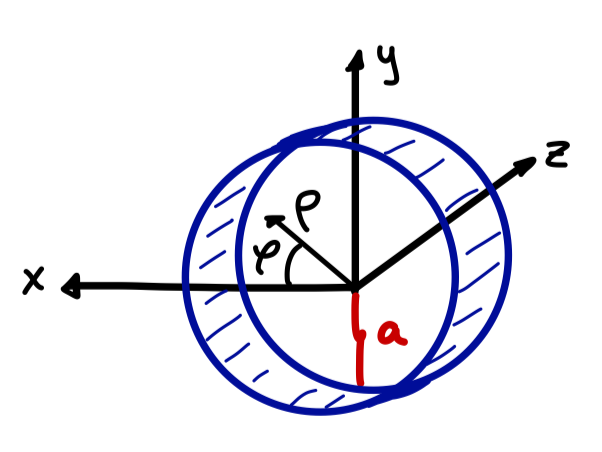
\includegraphics[width=8cm]{img/Guia_de_onda_circular.jpg}
\end{center}

Al igual que en la gu\'ia rectangular, podemos calcular $E_z$ y $H_z$ resolviendo la ecuaci\'on de onda, y despu\'es obtener $\vec{E}_t$ y $\vec{H}_t$ a partir de $E_z$ y $H_z$. Es importante prestar arenci\'on a la inclusi\'on de los factores de forma de este sistema de coordenadas, que en cartesianas se obviaba, por valer todos 1.

\subsubsection{Modos TE en la Gu\'ia de Onda Cil\'indrica}

Partiendo de la condici\'on $E_z = 0$, la ecuaci\'on de onda que buscamos resolver es:
$$\nabla^2 H_z + k^2 H_z =0$$

Que, en coordenadas cil\'indricas, queda como:
$$\cfrac{\partial^2 H_z}{\partial \rho^2} +\cfrac{1}{\rho}\cdot\cfrac{\partial H_z}{\partial \rho}+\cfrac{1}{\rho^2} \cdot\cfrac{\partial^2 H_z}{\partial \varphi^2} + k^2_c H_z = 0$$

Expresamos la funci\'on $H_z(\rho, \varphi)$ como producto $R(\rho)\cdot F(\varphi)$
$$F\cfrac{\partial^2 R}{\partial \rho^2} +F\cfrac{1}{\rho}\cdot\cfrac{\partial R}{\partial \rho}+R\cfrac{1}{\rho^2} \cdot\cfrac{\partial^2 F}{\partial \varphi^2} + k^2_c F\cdot R = 0$$

Multiplicando por $\cfrac{\rho^2}{R\cdot F}$ y reordenando:
$$\rho^2\cfrac{1}{R}\cfrac{\partial^2 R}{\partial \rho^2} +\rho\cfrac{1}{R}\cdot\cfrac{\partial R}{\partial \rho} + k^2_c \rho^2 = -\cfrac{1}{F} \cdot\cfrac{\partial^2 F}{\partial \varphi^2}$$

Ahora los dos lados de la igualdad son ecuaciones diferenciales en variables ortogonales, por lo que la \'unica forma de cumplirse es suponer que ambas expresiones toman un valor constante, al que llamaremos $v^2$.

$$-\cfrac{1}{F} \cdot\cfrac{\partial^2 F}{\partial \varphi^2} = v^2$$
$$\rho^2\cfrac{1}{R}\cfrac{\partial^2 R}{\partial \rho^2} +\rho\cfrac{1}{R}\cdot\cfrac{\partial R}{\partial \rho} + k^2_c \rho^2 = v^2 \hspace{0.3cm}\rightarrow \hspace{0.3cm} \cfrac{\partial^2 R}{\partial \rho^2} +\cfrac{1}{\rho}\cdot\cfrac{\partial R}{\partial \rho} + R\left( k^2_c  - \cfrac{v^2}{\rho^2}\right) = 0$$

La primera ecuaci\'on se puede resolver como:

$$F(\varphi) = A_1\cos(n\varphi) +B_1\sen(n\varphi) \hspace{1cm} n \in [0,1,2...]$$

Mientras que la segunda es la llamada ecuaci\'on de Bessel, cuya soluci\'on es una combinaci\'on lineal de funciones de Bessel de 1\textsuperscript{a} y 2\textsuperscript{a} especie ($J_u$ e $Y_v$, respectivamente):
$$R(\rho) = C_1\cdot J_u(k_c\rho) + D_1\cdot Y_v(k_c\rho)$$
\begin{center}
	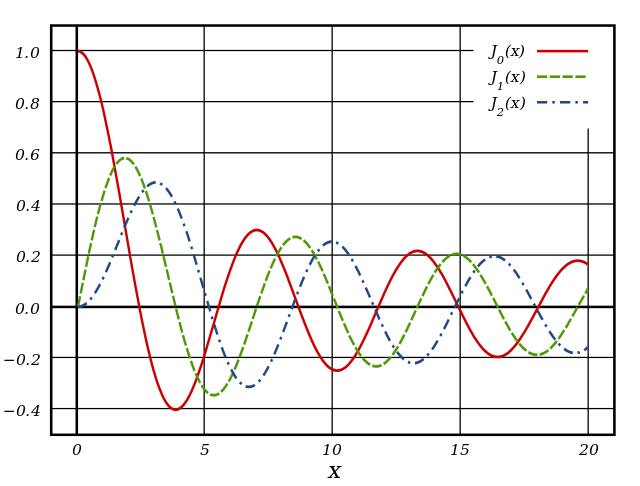
\includegraphics[width=7cm]{img/Bessel_de_primera_especie.png}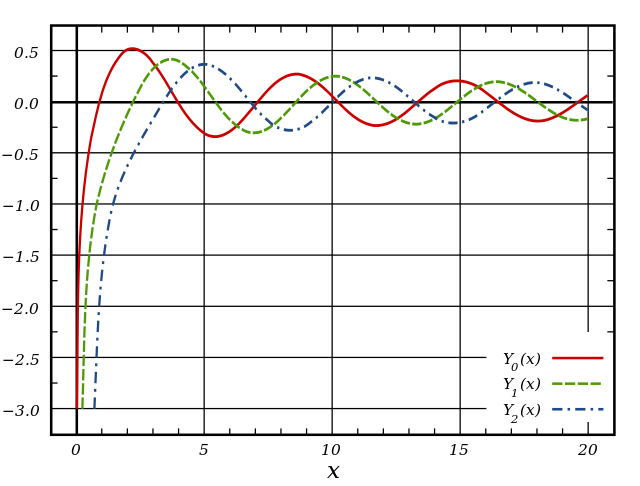
\includegraphics[width=7cm]{img/Bessel_de_segunda_especie.png}
\end{center}

La expresi\'on del campo queda pues como:
$$H_z = [A_1\cos(n\varphi) +B_1\sen(n\varphi)]\cdot[C_1\cdot J_u(k_c\rho) + D_1\cdot Y_V(k_c\rho)]$$

Como se observa en las gr\'aficas anteriores, las funciones de Bessel de 2\textsuperscript{a} especie ($Y_v$) divergen en el origen. Incluir cualquiera de estas funciones en nuestra expresi\'on resultar\'ia en un campo infinito en el centro de la l\'inea, lo cual es imposible, conque:
$$D_1 = 0 \hspace{0.3cm}\rightarrow \hspace{0.3cm} H_z = C_1[A_1\cos(n\varphi) +B_1\sen(n\varphi)] J_u(k_c\rho)$$

A continuaci\'on, observamos que la funci\'on seno y coseno interfieren en t\'erminos de m\'aximos  y m\'inimos, anular uno u otro depender\'a de la elecci\'on del origen\footnote{Para el caso $n=0$, se escoger\'a siempre anular el seno, a fin de no anular el campo. No importar\'a el origen de para $\varphi$, ya que no habr\'a variaci\'on en esa direcci\'on.} para $\varphi$. Teniendo esto en cuenta y expresando los coeficientes restantes como producto, $A$, el campo queda:
$$H_z = A J_u(k_c\rho)\left( \begin{array}{l}
        \cos(n\varphi) \\
        \sen(n\varphi)\end{array} \right)$$
        
El siguiente paso es aplicar la condici\'on de pared el\'ectrica en el contorno de la l\'inea, expresada en t\'erminos de campo magn\'etico:
$$\cfrac{\partial H_z}{\partial\rho}\bigg|_{\rho = a} = A J'_u(k_c\rho)\left( \begin{array}{l}
        \cos(n\varphi) \\
        \sen(n\varphi)\end{array} \right)\Bigg|_{\rho = a} = A J'_u(k_c a)\left( \begin{array}{l}
        \cos(n\varphi) \\
        \sen(n\varphi)\end{array} \right)=0$$

Puesto que ni $A$ ni $k_c$ pueden valer 0, y podemos omitir la parte dependiente de $\varphi$:
$$J'_u(k_c a) = 0$$
	
	La funci\'on $J'_u$ se anula en los m\'aximos y m\'inimos de la funci\'on de Bessel de la que procede; los valores de estos puntos se encuentran calculados en tablas, y se denotan como $P'_{nl}$, donde $n$ representa el orden de la funci\'on de Bessel, y $l$ es la ordinalidad del cero.
$$k_c a = P'_{nl} \hspace{0.3cm}\rightarrow \hspace{0.3cm} k_c = \cfrac{P'_{nl}}{a}$$

\begin{center}
  \begin{tabular}{ r | r | r | r }
    n & $P'_{n1}$ & $P'_{n2}$ & $P'_{n3}$\\ \hline
    0 & 3,832 & 7,016 & 10,174\\ \hline
    1 & 1,841 & 5,331 & 8,536\\ \hline
    2 & 3,054 & 6,706 & 9,970\\
  \end{tabular}
\end{center}

Teniendo esto en cuenta: 
$$H_z = A J_u\left(\cfrac{P'_{nl}}{a}\rho\right)\left( \begin{array}{l}
        \cos(n\varphi) \\
        \sen(n\varphi)\end{array} \right) e^{-j\beta z}$$
        
Y a partir de $H_z$ podemos calcular el resto de los campos:
$$\begin{array}{rr@{}l}
        H_\rho = & \cfrac{-j\beta a}{P'_{nl}} A J'_u\left(\cfrac{P'_{nl}}{a}\rho\right) & \left( \begin{array}{l}
        	\cos(n\varphi) \\
        	\sen(n\varphi)
        \end{array} \right) e^{-j\beta z}\\
        H_\varphi=  &  \cfrac{-j\beta a^2n}{P'^2_{nl}\rho} A J_u\left(\cfrac{P'_{nl}}{a}\rho\right) & \left( \begin{array}{r}
        	-\sen(n\varphi) \\
        	\cos(n\varphi)
        \end{array} \right) e^{-j\beta z}\\
        E_\rho =&  \cfrac{-j\omega\mu a^2n}{P'^2_{nl}\rho} A J_u\left(\cfrac{P'_{nl}}{a}\rho\right) & \left( \begin{array}{r}
        	-\sen(n\varphi) \\
        	\cos(n\varphi)
        \end{array} \right) e^{-j\beta z}\\
        E_\varphi = & \cfrac{-j\omega\mu a}{P'_{nl}} AJ'_u\left(\cfrac{P'_{nl}}{a}\rho\right) & \left( \begin{array}{l}
        	\cos(n\varphi) \\
        	\sen(n\varphi)
        \end{array} \right) e^{-j\beta z} \end{array}$$
        
La constante de propagaci\'on $\gamma = j\beta$ se calcula como:

$$\gamma^2 = k^2_{cnl} -k^2 = \left(\cfrac{P'_{nl}}{a}\right)^2 - \omega^2\mu\varepsilon$$

Y la frecuencia de corte:

$$f_c = \cfrac{P'_{nl}}{2\pi a\sqrt{\mu\varepsilon}}$$

Consultando la tabla de $P'_{nl}$, vemos que la frecuencia de corte m\'as baja es la del modo $TE_{11}$.

\subsubsection{Modos TM en la Gu\'ia de Onda Circular}

Partiendo de que $H_z = 0$, desarrollamos  la ecuaci\'on $\nabla^2 E_z + k^2 E_z =0$ (en coordenadas cil\'indricas) para obtener:

$$\cfrac{\partial^2 E_z}{\partial \rho^2} +\cfrac{1}{\rho}\cdot\cfrac{\partial E_z}{\partial \rho}+\cfrac{1}{\rho^2} \cdot\cfrac{\partial^2 E_z}{\partial \varphi^2} + k^2_c E_z = 0$$

Despu\'es de descomponer $E_z(\rho, \varphi)$ como el producto $R(\rho)\cdot F(\varphi)$, nos encontramos en la misma situaci\'on que en el an\'alisis de modos $TE$. Aplicando la misma l\'ogica, ignoramos las funciones de Bessel de 2\textsuperscript{a} especie, y escogemos seno o coseno (seg\'un convenga para el origen de coordenadas empleado). La expresi\'on de $E_z$ queda:

$$E_z = A J_u(k_c\rho)\left( \begin{array}{l}
        \cos(n\varphi) \\
        \sen(n\varphi)\end{array} \right)$$

Aplicando la condici\'on de pared el\'ectrica en el contorno de la l\'inea:

$$E_z\big|_{\rho = a} = A J_u(k_c\rho)\left( \begin{array}{l}
        \cos(n\varphi) \\
        \sen(n\varphi)\end{array} \right)\Bigg|_{\rho = a} = A J_u(k_c a)\left( \begin{array}{l}
        \cos(n\varphi) \\
        \sen(n\varphi)\end{array} \right)=0$$
        
Puesto que ni $A$ ni $k_c$ pueden valer 0, y podemos omitir la parte dependiente de $\varphi$:
$$J_u(k_c a) = 0 \hspace{0.3cm}\rightarrow \hspace{0.3cm} k_c a = P_{nl} \hspace{0.3cm}\rightarrow \hspace{0.3cm} k_c = \cfrac{P_{nl}}{a}$$

Donde $P_{nl}$ es el l-\'esimo cero de la n-\'esima funci\'on de Bessel de 1\textsuperscript{a} especie. Sus valores num\'ericos se pueden consultar en tablas.

\begin{center}
  \begin{tabular}{ r | r | r | r }
    n & $P_{n1}$ & $P_{n2}$ & $P_{n3}$\\ \hline
    0 & 2,405 & 5,520 & 8,654\\ \hline
    1 & 3,832 & 7,016 & 10,174\\ \hline
    2 & 5,135 & 8,417 & 11,620\\
  \end{tabular}
\end{center}

El modo $TM$ con menor frecuencia de corte es el $TM_{01}$.

\subsubsection{Propagaci\'on de Modos TE y TM en la Gu\'ia de Onda Circular}

Puesto que las frecuencias de corte de los modos $TE$ y $TM$ se calculan con los ceros de funciones diferentes ($J'_u$ y $J_u$, respectivamente), no existir\'an modos degenerados.
$$f_{cTE} = \cfrac{P'_{nl}}{2\pi a\sqrt{\mu\varepsilon}} \hspace{1cm} f_{cTM} = \cfrac{P_{nl}}{2\pi a\sqrt{\mu\varepsilon}}$$

Puesto que el menor valor de $P'_{nl}$ \'o $P_{nl}$ es $P'_{11}$, el primer modo en transmitirse, y por lo tanto el modo fundamental, es el modo $TE_{11}$. Para calcular su margen din\'amico, empleamos el valor del siguiente modo en propagarse, el $TM_{01}$:

$$\cfrac{f_{cTM01}}{f_{cTE11}} = \cfrac{P_{01}}{P'_{11}} = \cfrac{2,405}{1,841} \approx 1,3$$

Las impedancias caracter\'isticas de los modos vienen dadas por:

$$z_{TE} = \cfrac{?}{?} \hspace{1cm} z_{TM} = \cfrac{?}{?}$$

\subsubsection{Potencia, P\'erdidas y Atenuaci\'on en la Gu\'ia Circular}

La potencia transmitida por los modos TE y TM se calcula como:

$$P_{TE} =\cfrac{1}{2z_{TE}}\iint_S |\vec{E_t}|^2 dS = \cfrac{\eta^2}{2z_{TE}}\left(\cfrac{f}{f_c}\right)^2 \iint_S |\vec{H_z}|^2 dS$$

$$P_{TM} =\cfrac{z_{TM}}{2}\iint_S |\vec{H_t}|^2 dS = \cfrac{z_{TM}}{2\eta^2}\left(\cfrac{f}{f_c}\right)^2 \iint_S |\vec{E_z}|^2 dS$$

Las componentes del coeficiente de p\'erdidas, $\alpha = \alpha_c +\alpha_d$ se obtienen de la forma:
$$
\begin{array}{rl}
	\alpha_{cTE} = & \cfrac{R_S}{a\eta\sqrt{1-\left(\cfrac{f}{f_c}\right)^2}} \left[\left(\cfrac{f}{f_c}\right)^2 + \cfrac{n^2}{P'^2_{nl} -n^2}\right]\\
	\alpha_{cTM} = & \cfrac{R_S}{a\eta\sqrt{1-\left(\cfrac{f}{f_c}\right)^2}}\\
	\alpha_d = & \cfrac{k\tan(\delta)}{2\sqrt{1-\left(\cfrac{f}{f_c}\right)^2}}
\end{array}
$$


\subsection{El Cable Coaxial}

El cable coaxial consta de 2 conductores cil\'indricos conc\'entricos (el interno de radio $b$, y el externo de radio $a$). Asumiremos que la malla conductora externa tiene un espesor mucho mayor que la profundidad de penetraci\'on del conductor ($\delta$), lo que evita radiaci\'on al exterior e interferencias en el interior. Al presentar 2 conductores a diferente potencial, puede transmitir modos TEM, por lo que se emplea desde frecuencias muy bajas.

$$
	Cable\_coaxial.jpg
$$

\subsubsection{Funcionamiento como LT}
Los valores de algunos par\'ametrso de inter\'es del cable coaxial:
\begin{itemize}
	\item C?\footnote{Duda: ni puta idea de lo que significan (ni para qu\'e se usan, pero eso es irrelevante) la mitad de estos par\'ametros.}
	\item Impedancia caracter\'istica
	\item Resistencia
	\item Coeficiente de p\'erdidas por conductor
\end{itemize}

\subsubsection{Modos TEM en el Cable Coaxial}

\subsubsection{Modos TM en el Cable Coaxial}

\subsubsection{Modos TE en el Cable Coaxial}

\section{Resonancia}

\subsection{Introducci\'on}

Los circuitos resonantes son de vital importancia en multitud de aplicaciones, entre otras:
\begin{itemize}
	\item Amplificadores
	\item Filtros
	\item Aisladores
	\item Frecuenci\'ometros
\end{itemize}

Pueden implementarse mediante elementos concentrados, l\'ineas de transmisi\'on, o cavidades resonantes. Estas \'ultimas presentan beneficios tales como:
\begin{itemize}
	\item Resonancias muy selectivas
	\item Factores de calidad elevados
	\item Anchos de banda muy estrechos
\end{itemize}

\subsubsection{El Factor de Calidad ($Q$)}

El factor de calidad es una medida del rendimiento con que un sistema almacena energ\'ia al ser recorrido por una corriente alterna, y es un par\'ametro que interesa aumentar.
$$Q=2\pi\cfrac{U_{\text{MaxAlm}}}{U_{\text{dis}}}$$

Donde $U_{\text{MaxAlm}}$ es la energ\'ia m\'axima almacenada por el circuito, y $U_{\text{dis}}$ es la energ\'ia disipada durante un per\'iodo $T$. Llamando $P_m$ a la potencia media disipada, queda:

$$Q=2\pi\cfrac{U_{\text{MaxAlm}}}{P_m T} = \omega\cfrac{U_{\text{MaxAlm}}}{P_m}$$

El factor de calidad es inversamente proporcional al ancho de banda de resonancia, por lo que factores de calidad altos resultan en resonancias selectivas. Las l\'ineas de transmisi\'on t\'ipicamente presentan factores de calidad comprendidos entre 100 y 500, mientras que con las cavidades podemos esperar valores de 10000 a 20000.

\subsection{La Cavidad Rectangular}

Se obtiene una cavidad resonante rectangular cuando se cortocircuitan los extremos de una gu\'ia rectangular de dimensiones $a$ y $b$ con placas conductoras separadas por una distancia $d$:
\begin{center}
	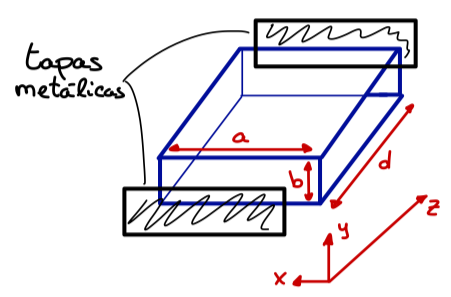
\includegraphics[width=8cm]{img/Cavidad_rectangular.jpg}
\end{center}

Partiendo de la funci\'on de campo del modo fundamental, $TE_{10}$, aplicaremos las nuevas condiciones de contorno impuestas por los nuevos cortocircuitos ($z = 0$ y $z = d$).
$$E_y = A\sen\left(\cfrac{\pi x}{a}\right) e^{-\gamma z} \hspace{1cm} (E_z = E_x =0)$$

Teniendo en cuenta que la variaci\'on seg\'un $z$ se puede expresar como suma de la onda regresiva y progresiva:
$$E_y = (A^+ e^{-j\beta z} + A^- e^{j\beta z})\sen\left(\cfrac{\pi x}{a}\right)$$

Aplicamos la condici\'on de contorno $E_y\big|_{z=0} = 0$:
$$E_y\big|_{z=0} = (A^+ + A^-)\sen\left(\cfrac{\pi x}{a}\right) = 0$$

Puesto que no podemos manipular la parte que depende de $x$, $A^+ = -A^-$:
$$E_y = (A^+ e^{-j\beta z} - A^+ e^{j\beta z})\sen\left(\cfrac{\pi x}{a}\right) = A^+ (e^{-j\beta z} - e^{j\beta z})\sen\left(\cfrac{\pi x}{a}\right)$$
$$E_y = -2jA^+ \sen(\beta z) \sen\left(\cfrac{\pi x}{a}\right)$$

A esta expresi\'on le aplicamos la segunda condici\'on de pared el\'ectrica, $E_y\big|_{z=d} = 0$:
$$E_y\big|_{z=d} = -2jA^+ \sen(\beta d) \sen\left(\cfrac{\pi x}{a}\right) = 0$$

Ignorando la parte que depende de x, $sen(\beta d) = 0$:
$$\beta d = p\pi \hspace{0.3cm} \rightarrow \hspace{0.3cm} \beta = \cfrac{p\pi}{d} \hspace{1cm} p = [1,2,3,...]$$

Esta restricci\'on sobre la constante de fase ($\beta$) representa la selectividad en frecuencia de la cavidad: el campo s\'olo existe en las frecuencias que cumplan la condici\'on anterior, en vez de aparecer a partir de una frecuencia umbral, como en las gu\'ias no cortocircuitadas. Para hallar la(s) frecuencia(s) de resonancia del modo $TE_{10}$:
$$\beta^2 = k^2 - k_c^2 \hspace{0.3cm} \rightarrow \hspace{0.3cm} \left(\cfrac{p\pi}{d}\right)^2 = (2\pi f_r)^2 \mu\varepsilon -\left(\cfrac{\pi}{a}\right)^2$$
$$f_r = \cfrac{1}{2\sqrt{\mu\varepsilon}}\sqrt{\left(\cfrac{1}{a}\right)^2 - \left(\cfrac{p}{d}\right)^2}$$

Los valores de $p$ producen las frecuencias de resonancia del modo $TE_{10}$, $f_{rTE_{10}p}$. De forma general, para un modo $mn$ en una cavidad rectangular, los n\'umeros de onda de resonancia se calculan como:
$$k_{rmnp} = \sqrt{\left(\cfrac{\pi m}{a}\right)^2 +\left(\cfrac{\pi n}{b}\right)^2+\left(\cfrac{\pi p}{d}\right)^2}$$

\subsubsection{Factor de Calidad}

Para calcular el factor de calidad de una cavidad, debemos considerar las p\'erdidas provenientes de la utilizaci\'on de conductores imperfectos ($\sigma < \infty$) y diel\'ectricos no ideales ($\sigma \neq 0$). Partiendo de la definici\'on:
$$Q=  \omega\cfrac{U_{\text{MaxAlm}}}{P_m}$$

La energ\'ia almacenada en la cavidad es la suma de las energ\'ias asociadas al campo el\'ectrico y al magn\'etico ($U=U_E+U_M$), que en r\'egimen de resonancia son iguales ($U = 2 U_E = 2 U_M$).
$$U_E = \cfrac{\varepsilon}{4} \iiint_V |\vec{E}|^2 dV \hspace{1cm} U_M = \cfrac{\mu}{4} \iiint_V |\vec{H}|^2 dV$$


Para la resonancia $TE_{101}$ ($m = 1, n = 0, p = 1$), es m\'as sencillo comenzar por el campo el\'ectrico:
$$U = 2U_E = \cfrac{\varepsilon}{2} \iiint_V |\vec{E}_y|^2 dV = $$
$$\cfrac{\varepsilon}{2} \int_0^a\int_0^b\int_0^d (2A^+)^2 \sen^2 \left(\cfrac{\pi x}{a}\right) \sen^2 \left(\cfrac{\pi z}{d}\right) dxdydz = \cfrac{(A^+)^2 \varepsilon a b d}{2}$$

Para calcular la potencia disipada, tenemos en cuenta la debida a las p\'erdidas en conductor ($P_{lc}$) y en diel\'ectrico ($P_{ld}$). Comenzando por $P_{lc}$:
$$P_{lc} = \cfrac{R_s}{2} \oint_\text{contorno} |\vec{J}_s|^2 dl = \cfrac{R_s}{2} \iint_S |\vec{H}_{tS}|^2 dS = $$
$$\cfrac{R_s}{2}\left[ 2 \int_0^a \int_0^b |\vec{H}_{x}|_{z=0}^2 dxdy +2 \int_0^b\int_0^d |\vec{H}_{z}|_{x\footnote{Yo creo que es x}=0}^2 dydz\right]$$

Lo cual\footnote{En el caso gen\'erico, habr\'ia que calcular la integral de superficie de $\hat{n}\times\vec{H}$ en todos los contornos de la gu\'ia, aunque aqu\'i hemos obviado $\int_0^a \int_0^d |\vec{H}_{y}|_{y=0}^2$, ya que $E_y = 0$.}, suponiendo p\'erdidas bajas, se simplifica (de una forma que no demostraremos) para llegar a:

$$P_{lc} = \cfrac{(A^+)^2 R_s \lambda^2}{2\eta^2}\left[\cfrac{ab}{d^2} + \cfrac{bd}{a^2} +\cfrac{1}{2}\left(\cfrac{a}{d} + \cfrac{d}{a}\right)\right]$$

Las p\'erdidas en diel\'ectrico, $P_{ld}$, se calculan a partir de la conductividad del mismo, $\sigma_e = \omega\varepsilon' \varepsilon_0 tg(\delta)$, que usamos en:
$$P_{ld} = \cfrac{1}{2}\iiint_V \vec{J}\times\vec{E}^* dV = \cfrac{\sigma_e}{2}\iiint_V |\vec{E}_y|^2 dV = \cfrac{(A^+)^2 \varepsilon ''\varepsilon_0 a b d}{2}$$

De forma gen\'erica\footnote{Duda: Espero que sea gen\'erico, porque jo-der.}, las contribuciones de los diel\'ectricos y conductores imperfectos a un factor de calidad real, no infinito, se pueden caracterizar descomponiendo $Q$ de la forma:

$$\cfrac{1}{Q} = \cfrac{1}{Q_c} +\cfrac{1}{Q_d} \hspace{1cm} Q= \cfrac{Q_cQ_d}{Q_c + Q_d}$$

$$Q_c = \cfrac{\pi\eta}{2R_s} \cdot \cfrac{b(a^2+d^2){3/2}}{ad(a^2+d^2) + 2b(a^3+d^3)} \hspace{1cm} Q_d = \cfrac{1}{\tan\delta}$$


\subsection{La Cavidad Circular}

La cavidad circular se obtiene cortocircuitando los extremos de una gu\'ia circular a una distancia $d$, an\'alogamente a la cavidad rectangular.
\begin{center}
	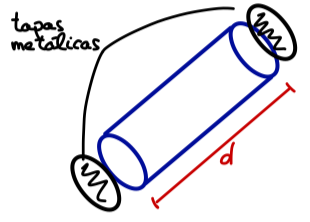
\includegraphics[width=7cm]{img/Cavidad_circular.jpg}
\end{center}

Partiendo de la expresi\'on del campo en coordenadas cil\'indricas, a\~nadimos las ondas progresiva y regresiva a la dependencia seg\'un $z$:
$$\vec{E} = (A^+ e^{-j\beta z} - A^+ e^{j\beta z}) \vec{E_t} (\rho, \varphi)$$

Aplicando la condici\'on de contorno en $z = 0$:
$$\vec{E}_t \big|_{z=0} = (A^+ + A^-) \vec{E_t} (\rho, \varphi) \hspace{0.3cm} \rightarrow \hspace{0.3cm} A^+ = -A^-$$
$$\vec{E} = -2jA^+ \sen(\beta z) \vec{E}_t (\rho, \varphi)$$

Y en $z = d$:
$$ \vec{E}_t \big|_{z=d}\vec{E} = -2jA^+ \sen(\beta d) \vec{E}_t (\rho, \varphi) = 0 \hspace{0.3cm} \rightarrow \hspace{0.3cm} \sen(\beta d) = 0$$
$$\beta d = q\pi \hspace{0.3cm} \rightarrow \hspace{0.3cm} \beta = \cfrac{q\pi}{d} \hspace{1cm} q = [1,2,3,...]$$

Obtenemos la selectividad en frecuencia de la cavidad. La frecuencia de resonancia se obtiene empleando las frecuencias de corte de cada modo, por lo que para modos $TE$ y $TM$ gen\'ericos:
$$f_{rTE_{nl}q} = \cfrac{1}{2\pi\sqrt{\mu\varepsilon}} \sqrt{\left(\cfrac{p'_{nl}}{a}\right)^2 + \left(\cfrac{q\pi}{d}\right)^2}$$
$$f_{rTM_{nl}q} = \cfrac{1}{2\pi\sqrt{\mu\varepsilon}} \sqrt{\left(\cfrac{p_{nl}}{a}\right)^2 + \left(\cfrac{q\pi}{d}\right)^2}$$

\subsubsection{Factor de Calidad}

Omitiendo los c\'alculos y demostraciones, las aportaciones de los conductores y diel\'ectricos al factor de calidad, $Q_c$ y $Q_d$, son:

$$Q_d = \cfrac{1}{\tan\delta} \hspace{1cm} Q_c = \cfrac{(ka)^3 \eta a d\footnote{Duda: esto no tiene puto sentido}}{4 p'_{nl} R_s} \cdot \cfrac{1-\left(\cfrac{u?}{p'_{nl}}\right)^2}{\cfrac{ad}{2}\left[1+\left(\cfrac{\beta a n}{p'_{nl}}\right)^2\right]+\left(\cfrac{\beta a }{p'_{nl}}\right)^2 \left(1-\cfrac{n^2}{p'nl}\right)}$$


\section{An\'alisis de Redes}

\subsection{Matriz de Dispersi\'on $[S]$}

La matriz de dispersi\'on surge como respuesta a la necesidad de analizar circuitos en la banda de microondas. Consideraremos un circuito al que se podr\'an conectar $n$ componentes, mediante l\'ineas de transmisi\'on, en cada uno de los denominados accesos.

$$\left(\begin{array}{c}
	V_1 \\
	V_2 \\
	\vdots \\
	V_n
\end{array}\right)
=
\left(\begin{array}{cccc}
	z_{11} & z_{12} & \cdots & z_{1n} \\
	z_{21} & z_{22} & \cdots & z_{2n} \\
	\vdots & \vdots & \ddots & \vdots \\
	z_{n1} & z_{n2} & \cdots & z_{nn}
\end{array}
\right)
\left(\begin{array}{c}
	I_1 \\
	I_2 \\
	\vdots \\
	I_n
\end{array}\right)$$

En cada una de dichas l\'ineas de transmisi\'on es necesario fijar un plano de referencia en el que medir las variables de inter\'es ($V$, $I$), lo cual presenta problemas end\'emicos a la banda de microondas:

\begin{itemize}
	\item La peque\~na longitud de onda provoca variaci\'on sustancial de los par\'ametros medidos con desplazamientos peque\~nos en la direcci\'on de propagaci\'on.
	\item Los circuitos abiertos y cortocircuitos empleados en mediciones presentan imperfecciones que tienden a funcionar como antenas, radiando energ\'ia y falseando la medici\'on.
	\item Cuando se consiguen, estos cortocircuitos o circuitos abiertos estables tienden a no estar en el plano deseado.
	\item Incluso salvando los obst\'aculos anteriores, los componentes activos podr\'ian da\~nar el dispositivo que queremos caracterizar.
\end{itemize}

Para poner soluci\'on a los problemas anteriores, se resorta a la medici\'on de la amplitud de la onda progresiva en la LT conectada al acceso. Por convenio, y a lo largo de todo el tema, consideraremos como direcci\'on positiva la de entrada a la red, y las variables se normalizar\'an respecto a la caracter\'istica de la l\'inea\footnote{Normalmente la impedancia de todas las l\'ineas de entrada a la red ser\'a la misma.} ($z_{0i}$). Algunos ejemplos:

$$\begin{array}{lll}
	a_i = \overline{V}_i^+ = \cfrac{V_i^+}{\sqrt{z_{0i}}} & \overline{V}_i = \cfrac{V_i}{\sqrt{z_{0i}}} &  \overline{V}_i = a_i + b_i\\
	b_i = \overline{V}_i^- = \cfrac{V_i^-}{\sqrt{z_{0i}}} & \overline{I}_i = \sqrt{z_{0i}} \cdot I_i &  \overline{I}_i = a_i - b_i
\end{array}$$

Asociadas a las ondas de tensi\'on en las LT, se encuentran sus potencias:

$$P_i^+ = \cfrac{|V_i^+|^2}{2z_{0i}} = \cfrac{1}{2} |a_i|^2 \hspace{1cm} P_i^-  = \cfrac{|V_i^-|^2}{2z_{0i}} = \cfrac{1}{2} |b_i|^2$$

Finalmente, la matriz de dispersi\'on es la que relaciona los par\'ametros $a$ y $b$ como $[b] = [S][a]$:

$$\left(\begin{array}{c}
	b_1 \\
	b_2 \\
	\vdots \\
	b_n
\end{array}\right)
=
\left(\begin{array}{cccc}
	S_{11} & S_{12} & \cdots & S_{1n} \\
	S_{21} & S_{22} & \cdots & S_{2n} \\
	\vdots & \vdots & \ddots & \vdots \\
	S_{n1} & S_{n2} & \cdots & S_{nn}
\end{array}
\right)
\left(\begin{array}{c}
	a_1 \\
	a_2 \\
	\vdots \\
	a_n
\end{array}\right)$$

Individualmente, podemos definir $S_{ji}$ como:

$$S_{ji} = \cfrac{b_j}{a_i}\bigg|_{a_k = 0} \hspace{4mm} \forall \hspace{2mm} k \neq i$$

Anular $a_k$ excepto en $k=i$ significa limitar las ondas incidentes \'unicamente al acceso $i$. Esto se consigue reemplazando las fuentes por impedancias iguales a la caracter\'istica de la l\'inea, $z_{0k}$, lo cual impide que las ondas regresivas $b_k$ se transmitan por ella volviendo a la red como progresivas. Esto es lo que se conoce como un acceso terminado (es importante se\~nalar que la condici\'on de acceso terminado no depende del plano de referencia, ya que los cambios de fase no afectan a la onda que no se transmite).

\vspace{0.3cm}

La definici\'on anterior implica que $S_{ji}$ puede verse como el coeficiente de transmisi\'on del acceso $i$ al acceso $j$, y cuando $i = j$, $S_{ii}$ corresponde al coeficiente de reflexi\'on en el acceso $i$ (siempre con los dem\'as terminados).

\vspace{0.3cm}

A partir de la matriz de dispersi\'on, las matrices de impedancia y admitancia (normalizadas) se pueden obtener como:

$$\overline{[z]} = (1+[S])(1-[S])^{-1} \hspace{1cm} \overline{[Y]} = (1-[S])(1+[S])^{-1}$$

Y a la inversa:

$$[S] = (\overline{[z]} +1)(\overline{[z]} -1)^{-1} \hspace{1cm} [S] = (1-\overline{[Y]})(1+\overline{[Y]})^{-1}$$

\subsubsection{Ejemplos}

\subsection{Propiedades de la Matriz de Dispersi\'on}

En esta secci\'on veremos qu\'e relaci\'on hay entre las caracter\'isticas f\'isicas de una red y las caracter\'isticas matem\'aticas de su matriz de dispersi\'on.

\subsubsection{Red Pasiva}

Una red pasiva es aquella que no posee la capacidad de generar potencia, y su matriz de dispersi\'on cumple que:

$$|S_{ji}| \leq 1 \hspace{0.7cm} \forall\hspace{0.1cm} i, j$$

A esta condici\'on se llega partiendo de la definici\'on $b = sa$:

$$b_i = S_{ji} a_j \hspace{0.3cm} \rightarrow \hspace{0.3cm} |b_i|\rightarrow = |S_{ji}||a_j| \hspace{0.3cm} \rightarrow \hspace{0.3cm} \left(\cfrac{1}{2}|b_i|^2 \right)= |S_{ji}|^2 \left(\cfrac{1}{2}|a_j|^2\right)$$

Las expresiones entre par\'entesis corresponden a las potencias saliente y entrante en los accesos $i$ y $j$, respectivamente. Para que se cumpla que la potencia saliente sea siempre menor a la entrante, debe ocurrir que $|S_{ji}|^2 \leq 1$, lo que equivale a nuestra expresi\'on inicial.

\subsubsection{Red sin P\'erdidas}

Las redes sin p\'erdidas constituyen un subconjunto de las redes pasivas, al no generar potencia, y por lo tanto sus matrices de dispersi\'on cumplen con las restricciones correspondientes, as\'i como:
$$\cfrac{1}{2}|b_i|^2 = \cfrac{1}{2}|a_i|^2 \hspace{0.3cm} \rightarrow \hspace{0.3cm} \sum_{i=1}^n \cfrac{1}{2}|b_i|^2 = \sum_{i=1}^n \cfrac{1}{2}|a_i|^2$$

O lo que es lo mismo, que la potencia saliente es igual a la potencia entrante. Esto tiene consecuencias adicionales, como que el m\'odulo de todos los vectores fila y columna de $S$ ha de valer 1:

$$\sum_{j=1}^n |S_{ij}|^2 = 1 \hspace{0.3cm} \sum_{j=1}^n |S_{ji}|^2 = 1 \hspace{0.3cm} \forall \hspace{0.1cm} i$$

Y que el producto de dos vectores fila o columna, habiendo conjugado uno de ellos, ha de ser 0:

$$\sum_{j=1}^n S_{ij}^* \cdot S_{kj} = 0 \hspace{0.3cm} \forall \hspace{0.1cm} i \neq k$$

\subsubsection{Red Rec\'iproca}

Se dice que una red es rec\'iproca cuando su matriz de dispersi\'on es sim\'etrica respecto a su diagonal principal:

$$S_{ij} = S_{ji} \hspace{0.3cm} \forall \hspace{0.1cm} i,j \hspace{1cm} S = S^t$$

Por la definici\'on de la matriz de impedancias y admitancias, estas propiedades tambi\'en se propagan\footnote{Las operaciones de suma, producto, inversi\'on y trasposici\'on de matrices sim\'etricas resultan en matrices sim\'etricas.} a ellas ($[z] = [z^t]$, $[Y] = [Y^t]$).

\subsubsection{Red Sim\'etrica}

Red sim\'etrica es aquella cuyos accesos presentan una simetr\'ia f\'isica:

$$S_{ii} =S_{jj} \hspace{0.3cm} \forall \hspace{0.1cm} i,j$$

Y por lo tanto, los elementos de su diagonal principal son iguales.

\subsection{Redes de dos Accesos}

Las redes de dos accesos se corresponden al concepto de cuadripolo, familiar del an\'alisis de curcuitos.

$$Cuadripolo.jpg \hspace{0.3cm} \rightarrow \hspace{0.3cm} S =\left(\begin{array}{cc}
	S_{11} & S_{12}\\
	S_{21} & S_{22}
\end{array}\right)$$

De su matriz de dispersi\'on podemos extraer las matrices de impedancia y admitancia, y con sus elementos ($z_{ji}$ e $Y_{ji}$) podemos implementar sus equivalentes en ``$\pi$'' y en ``$\tau$'':

$$Cuadripolo\_en\_pi.jpg \hspace{1cm} Cuadripolo\_en\_tau.jpg$$

Las matrices de impedancia y admitancia tambi\'en son \'utiles para caracterizar agregaciones de cuadripolos: al conectar cuadripolos en serie, como en la imagen, su matriz de impedancia conjunta es la suma de las impedancias de los cuadripolos individuales:

$$Cuadripolos\_en\_serie.jpg \hspace{0.3cm} \rightarrow \hspace{0.3cm} [z_T] = [z_A] + [z_B]$$

La matriz, de admitancias, por su parte, nos permite caracterizar f\'acilmente una conexi\'on de cuadripolos en paralelo:

$$Cuadripolos\_en\_paralelo.jpg \hspace{0.3cm} \rightarrow \hspace{0.3cm} [Y_T] = [Y_A] + [Y_B]$$

\paragraph{An\'alisis B\'asico del Cuadripolo}

Consideremos un cuadripolo al que, en su primer acceso, se le conecta un generador ($V_g$, $z_g$), y en su segundo acceso se le conecta una carga $z_L$, como en la imagen:

$$Cuadripolo\_cableado.jpg$$

De este an\'alisis gen\'erico buscamos obtener 3 caracter\'isticas importantes del cuadripolo:
\begin{itemize}
	\item Impedancia de entrada.
	\item Impedancia de salida.
	\item Ganancia de transferencia.
\end{itemize}

Para empezar, partimos de la definici\'on de la matriz de dispersi\'on, que relaciona las amplitudes de ondas entrantes y salientes:

$$\left(\begin{array}{c}
	b_1\\
	b_2
\end{array}\right)
=
\left(\begin{array}{cc}
	S_{11} & S_{12}\\
	S_{21} & S_{22}
\end{array}\right)
\left(\begin{array}{c}
	a_1\\
	a_2
\end{array}\right)
\hspace{0.3cm} \rightarrow \hspace{0.3cm}
\left\{\begin{array}{cc}
	b_1 = & a_1 S_{11} + a_2 S_{12}\\
	b_2 = & a_1 S_{21} + a_2 S_{22}
\end{array}\right.
$$

Puesto que en cada acceso hay una l\'inea de transmisi\'on conectando el elemento en cuesti\'on a la red, tendremos que tener en cuenta 2 factores de reflexi\'on en cada acceso. Llamendo $\rho_L$ al factor de reflexi\'on en carga, $\rho_g$ al de generador, y $\rho_{in}$ / $\rho_{out}$ a los factores de reflexi\'on de los accesos a la red:

$$\begin{array}{r@{}lr@{}l}
	\rho_L &=\cfrac{a_2}{b_2} = \cfrac{z_{L}-z_{02}}{z_{L}+z_{02}}& \rho_{out}&= \cfrac{b_2}{a_2} = \cfrac{1}{\rho_L}\\
	\rho_g &=\cfrac{a_1}{b_1} = \cfrac{z_{g}-z_{01}}{z_{g}+z_{01}}& \rho_{in} &= \cfrac{b_1}{a_1} = \cfrac{1}{\rho_g}
\end{array}$$

Una vez definidos los coeficientes de reflexi\'on, comenzamos el an\'alisis dividiendo la primera ecuaci\'on, obtenida de la matriz de dispersi\'on, entre $a_1$:

$$\cfrac{b_1}{a_1} = S_{11} + S_{12}\cfrac{a_2}{a_1} \hspace{0.3cm} \rightarrow \hspace{0.3cm} \rho_{in} = S_{11} + S_{12}\cfrac{a_2}{a_1}$$

Y la segunda entre $a_2$:

$$\cfrac{b_2}{a_2} = S_{21}\cfrac{a_1}{a_2} + S_{22} \hspace{0.3cm} \rightarrow \hspace{0.3cm} \rho_{out} = S_{21}\cfrac{a_1}{a_2} + S_{22}$$

De la 2\textsuperscript{a} ecuaci\'on podemos despejar $\cfrac{a_2}{a_1}$:

$$\cfrac{a_1}{a_2} = \cfrac{\rho_{out} - S_{22}}{S_{21}} \hspace{0.3cm} \rightarrow \hspace{0.3cm} \cfrac{a_2}{a_1} = \cfrac{S_{21}}{\rho_{out} - S_{22}}$$

Y sustituir lo obtenido en la 1\textsuperscript{a}:

$$\rho_{in} = S_{11} + S_{12}\cfrac{S_{21}}{\rho_{out} - S_{22}} = S_{11} + S_{12}\cfrac{S_{21}}{\cfrac{1}{\rho_L} - S_{22}}$$

$$\rho_{in} = S_{11} + \cfrac{S_{21}S_{12}\rho_L}{1 - S_{22}\rho_L}$$

De esta forma obtenemos una definici\'on de $\rho_{in}$ que no depende de las caracter\'isticas del generador. Teniendo en cuenta la impedancia de la l\'inea de entrada, $z_{01}$, podemos calcular:

$$z_{in} = z_{01}\cfrac{1+\rho_{in}}{1-\rho_{in}}$$

Con un desarrollo similar, podemos definir $\rho_{out}$ independientemente de la impedancia de carga, como:

$$\rho_{out} = S_{22} + \cfrac{S_{21}S_{12}\rho_g}{1 - S_{11}\rho_g}$$

Y usarlo para calcular la impedancia de salida:

$$z_{out} = z_{02}\cfrac{1+\rho_{out}}{1-\rho_{out}}$$

Finalmente, la ganancia de transferencia, se puede definir as\'i:

$$G_T = \cfrac{P_L}{P_{avg}}$$

Donde $P_L$ es la potencia entregada a la carga $z_L$, y $P_{avg}$ es la potencia que entregar\'ia a una carga $z_g^*$ en su lugar. Omitiendo la demostraci\'on, se calcula:

$$G_T = \cfrac{|S_{21}|^2 (1-|\rho_L|^2) (1-|\rho_g|^2)}{|(1-\rho_g S_{11})(1-\rho_L S_{22}) -S_{21}^2 \rho_L\rho_g|^2}$$

\subsubsection{Atenuadores}

Como su nombre permite adivinar, un atenuador es un sistema que reduce los niveles de se\~nal en un valor constante y prefijado desde su dise\~no. Si queremos implementar un atenuador en una red de 2 accesos, debemos considerar 2 premisas:
\begin{itemize}
	\item Tenemos que respetar las condiciones preexistentes de adaptaci\'on entre generador y carga.
	\item No debemos introducir desfases indeseados en la se\~nal (sobre todo si es dependiente\footnote{Duda: el desfase? la atenuaci\'on? la se\~nal?} de la frecuencia).
\end{itemize}

El atenuador que cumple estas 2 condiciones presenta una matriz de dispersi\'on de la forma:
$$S =\left(\begin{array}{cc}
	0 & e^{-\gamma}\\
	e^{-\gamma} & 0
\end{array}\right)$$

Forzar que $\gamma$ sea un n\'umero real puro evita los desfases indeseados, y anular $S_{11}$ y $S_{22}$ nos permite conservar la adaptaci\'on de carga y generador, puesto que (teniendo en cuenta que $\rho_L$ y $\rho_g$ valen 0 en situaci\'on de adaptaci\'on):

$$\rho_{out} = S_{22} + \cfrac{S_{21}S_{12}\rho_g}{1 - S_{11}\rho_g} = 0 + \cfrac{S_{21}S_{12}\cdot 0}{1 - 0\cdot0} = 0$$

$$\rho_{in} = S_{11} + \cfrac{S_{21}S_{12}\rho_L}{1 - S_{22}\rho_L} = 0 + \cfrac{S_{21}S_{12}\cdot 0}{1 - 0\cdot0} = 0$$

Las impedancias de entrada y salida corresponden a la caracter\'istica de cada l\'inea:

$$z_{in} = z_{01}\cfrac{1+\rho_{in}}{1-\rho_{in}} = z_{01} \hspace{1cm} z_{out} = z_{02}\cfrac{1+\rho_{out}}{1-\rho_{out}} = z_{02}$$

Y la ganancia de transferencia queda:

$$G_T = \cfrac{|S_{21}|^2 (1-|0|^2) (1-|0|^2)}{|(1-0 S_{11})(1-0 S_{22}) -S_{21}^2 \cdot 0|^2} = |S_{21}|^2 = e^{-2\gamma}$$

A partir de la ganancia, podemos calcular la atenuaci\'on (o p\'erdidas) en deciBelios:

$$L(\text{dB}) = -10 \log(G_T) = -20 \log(S_{21}) = -20 \log(e^{-\gamma}) = 20\gamma \log(e) \approx 8'686 \gamma$$


\subsubsection{Inversores de Impedancia y Admitancia}

Los inversores de impedancia son circuitos muy importantes en microondas. Se definen como un cuadripolo que, al conectarle una impedancia $z_L$ en un extremo, presentan en el otro la impedancia inversa (multiplicada por una constante). Lo mismo se puede decir de una admitancia.

$$z_{in} = \cfrac{k^2}{z_L} \hspace{1cm} Y_{in} = \cfrac{J^2}{Y_L} \hspace{1cm} k^2 = \cfrac{1}{J^2}$$

Siendo $J$ y $k$ n\'umeros reales positivos. Para caracterizar este cuadripolo, partimos de su matriz de impedancia, que definimos como sim\'etrica y rec\'iproca:

$$z =\left(\begin{array}{cc}
	0 & z_{12}\\
	z_{12} & 0
\end{array}\right)
\hspace{0.3cm} \rightarrow \hspace{0.3cm}
\left\{\begin{array}{cc}
	V_1 = & z_{12} I_2\\
	V_2 = & z_{12} I_1
\end{array}\right.$$

Con estas ecuaciones y la definici\'on del inversor, podemos aplicar que $z_{in} = \cfrac{V_1}{I_1}$ y que $z_{out} = - \cfrac{V_2}{I_2}$ para obtener:

$$\cfrac{V_1}{I_1} = \cfrac{-k^2}{V_2/I_2} \hspace{0.3cm} \rightarrow \hspace{0.3cm} -k^2 = z_{12}^2 \hspace{0.3cm} \rightarrow \hspace{0.3cm} z_{12} = \pm jk$$

Con un desarrollo similar se puede obtener que $Y_{12} = \pm jJ$. Se pueden, por lo tanto, implementar inversores en ``$\tau$'' y ``$\pi$'' empleando \'unicamente reactancias ($X$) o susceptancias ($B$) puras, respectivamente. En el caso del cuadripolo en ``$\tau$'', $z_{s} = \mp jX$ y $z_{p} = \pm jX$; para en cuadripolo en ``$\pi$'', $z_{s} = \mp jB$ y $z_{p} = \pm jB$.

$$Inversor\_en\_tau.jpg \hspace{1cm} Inversor\_en\_pi.jpg$$

Para calcular su matriz de dispersi\'on, $S_{11}$ (que, por simetr\'ia, ser\'a igual a $S_{22}$) se obtiene de su f\'ormula (como factor de reflexi\'on en el acceso 1, estando terminado el acceso 2), a la que se aplica la definici\'on del inversor:

$$S_{11} = \cfrac{z_{in} - z_0}{z_{in} + z_0} = \cfrac{k^2/z_L - z_0}{k^2/z_L + z_0} = \cfrac{k^2/z_0 - z_0}{k^2/z_0 + z_0} = \cfrac{k^2 - z_0^2}{k^2 + z_0^2}$$

Mediante un proceso similar, se puede obtener $S_{11}$ en t\'erminos de admitancias. Independientemente, llamaremos a este resultado $\gamma$:

$$S_{11} = \gamma = \cfrac{k^2 - z_0^2}{k^2 + z_0^2} = \cfrac{Y_0^2 - J^2}{Y_0^2 + J^2}$$

Una vez calculado $S_{11}$, la simetr\'ia implica que tenemos $S_{22}$, y la reciprocidad que s\'olo hace falta calcular un elemento m\'as, $S_{21}$.

$$S=\left(\begin{array}{cc}
	S_{11} & S_{12}\\
	S_{12} & S_{11}
\end{array}\right)$$

Para obtenerlo, usaremos la ausencia de p\'erdidas, que implica que el m\'odulo de filas y columnas ha de ser 1, y que el producto de una fila (o columna) por el conjugado de otra debe ser 0. Llamando $\gamma$ al elemento que ya hab\'iamos calculado, la matriz que cumple esto es:

$$S=\left(\begin{array}{cc}
	\gamma & \pm j\sqrt{1-\gamma^2}\\
	\\ %Por espacio, que si no queda feo%
	\pm j\sqrt{1-\gamma^2} & \gamma
\end{array}\right)$$



\subsection{Propiedades de Simetr\'ia}

\section{Divisores de Potencia y Acopladores direccionales}
\subsection{Redes de 3 Accesos}

\subsubsection{Propiedades}

Consideraremos estas redes (y en general, una red de cualquier tama\~no) como completamente adaptadas cuando los elementos de su diagonal principal ($S_{ii}$) ser\'an 0.
$$S = \left(\begin{array}{ccc}
	0 & a & b \\
	c & 0 & d \\
	e & f & 0
\end{array}\right)$$

Sin embargo, no puede existir una red pasiva, rec\'iproca, sin p\'erdidas y completamente adaptada. Para demostrar esto, consideremos su existencia, con una matriz de dispersi\'on de la siguiente forma:
$$S = \left(\begin{array}{ccc}
	0 & a & b \\
	a & 0 & c \\
	b & c & 0
\end{array}\right)$$

Considerando la propiedad de unietariedad:
$$\begin{array}{r@{=}l}
	|a|^2 + |b|^2 & 1 \\
	|a|^2 + |c|^2 & 1 \\
	|b|^2 + |c|^2 & 1
\end{array}$$

Restando la primera y la segunda ecuaci\'on, obtenemos $|b|^2 - |c|^2 = 0$, por lo que $b$ y $c$ son iguales en m\'odulo. Se puede obtener una expresi\'on para cualquier combinaci\'on de $a$, $b$, $c\ldots$ (y cualquier cantidad de par\'ametros de $S$, para cualquier tama\~no $N$). Como todo valdr\'a lo mismo, obtenemos:
$$a = \cfrac{1}{\sqrt{2}}$$

Multiplicando la 1\textsuperscript{a} fila por la 2\textsuperscript{a} conjugada, queda:
$$(0, a, b) \cdot (a, 0, c)^* = b \cdot c^* = 0$$

Si este producto se anula, alguno de sus factores lo hace, lo cual es incompatible con el c\'alculo anterior. Por lo tanto queda demostrado que nuestra red no puede ser pasiva, rec\'iproca, sin p\'erdidas y completamente adaptada.

\paragraph{Divisores de Potencia}

Para los divisores de potencia, la propiedad menos prioritaria es la adaptaci\'on, por lo que alg\'un elemento de su diagonal principal ($S_{ii}$) ser\'a no nulo. Considerando que, por dise\~no, un divisor de potencia s\'olo va a recibir potencia por un acceso ($S_{11}$, por convenio), los factores de reflexi\'on en las salidas pueden desadaptarse sin inconvenientes. La matriz $S$, de forma gen\'erica queda:
$$S = \left(\begin{array}{ccc}
	0 & a & b \\
	a & c & d \\
	b & d & e
\end{array}\right)$$

Por la definici\'on de $a$ y $b$ como factores de transmisi\'on, la expresi\'on $|a|^2 + |b|^2 = 1$ expresa el reparto de potencia entrante que sale por los accesos 2 y 3. Considerando un divisor sim\'etrico, el reparto de potencia es equitativo y los factores de reflexi\'on han de ser iguales, por lo que:
$$S = \left(\begin{array}{ccc}
	0 & a & a \\
	a & c & d \\
	a & d & c
\end{array}\right)$$
Aplicando la propiedad de unitariedad a la 1\textsuperscript{a} fila:
$$|a|^2 + |a|^2 = 1
\hspace{0.3cm} \rightarrow  \hspace{0.3cm}
a = \cfrac{1}{\sqrt{2}}$$

Aplicando la propiedad de unitariedad al producto de la 2\textsuperscript{a} y 3\textsuperscript{a} fila (conjugada), y a la 2\textsuperscript{a} por s\'i sola:
$$S = \left(\begin{array}{ccc}
	0 & \cfrac{1}{\sqrt{2}} & \cfrac{1}{\sqrt{2}} \\
	\cfrac{1}{\sqrt{2}} & c & d \\
	\cfrac{1}{\sqrt{2}} & d & c
\end{array}\right)
\hspace{0.3cm} \rightarrow  \hspace{0.3cm}
\begin{array}{l}
	\cfrac{1}{2} + 2cd = 0 \\
	\\
	\cfrac{1}{2} + c^2 +d^2 = 1
\end{array}
\hspace{0.3cm} \rightarrow  \hspace{0.3cm}
\begin{array}{l}
	c = \cfrac{1}{2} \\
	\\
	d = -\cfrac{1}{2}
\end{array}$$
$$S = \left(\begin{array}{ccc}
	0                   & \cfrac{1}{\sqrt{2}} & \cfrac{1}{\sqrt{2}} \\
	\cfrac{1}{\sqrt{2}} &  \cfrac{1}{2} & -\cfrac{1}{2} \\
	\cfrac{1}{\sqrt{2}} & -\cfrac{1}{2} &  \cfrac{1}{2}
\end{array}\right)$$

\paragraph{Combinadores de Potencia}

Un combinador de potencia cuya salida se encuentre en el acceso 1 puede presentar desadaptaci\'on en \'el, por lo que, asumiendo que queremos una igual contribuci\'on de los accesos 2 y 3:
$$S = \left(\begin{array}{ccc}
	a & b & b \\
	b & 0 & c \\
	b & c & 0
\end{array}\right)$$

Aplicando la condici\'on de unitariedad al producto de las fila 2 y 3:
$$(b , 0 , c) \cdot (b , c , 0)^* = b\cdot b^* = |b|^2 = 0
\hspace{0.3cm} \rightarrow  \hspace{0.3cm}
b = 0$$

Un coeficiente de transmisi\'on nulo implica que los accesos 2 y 3 est\'an aislados del 1, por lo que la red no puede funcionar como un combinador. Es, por lo tanto, inevitable que nuetro circuito combinador incurra en p\'erdidas.

\subsubsection{Divisores de Potencia}

\paragraph{Divisores con L\'ineas en $\cfrac{\lambda}{4}$}

En este apartado consideraremos 2 formas diferentes de implementar un divisor de potencia sim\'etrico empleando l\'ineas de transmisi\'on en $\lambda/4$, como se indica en las ilustraciones:
\begin{center}
	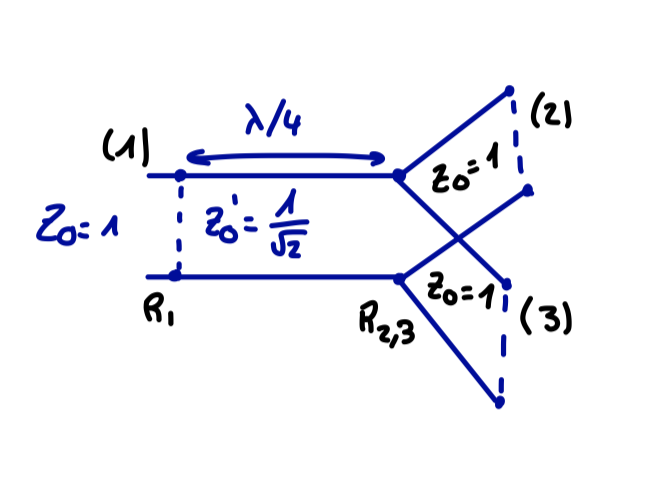
\includegraphics[width=7cm]{img/Divisor_en_lambda4_A.jpg}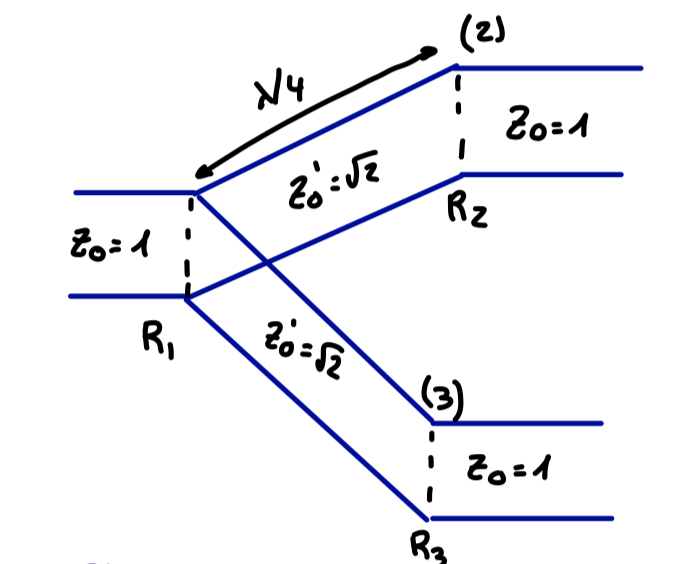
\includegraphics[width=7cm]{img/Divisor_en_lambda4_B.jpg}
\end{center}

Considerando una red con una \'unica l\'inea de transmisi\'on, suponemos que el acceso 1 est\'a adaptado y que su matriz de dispersi\'on es sim\'etrica y sin p\'erdidas.
\begin{center}
	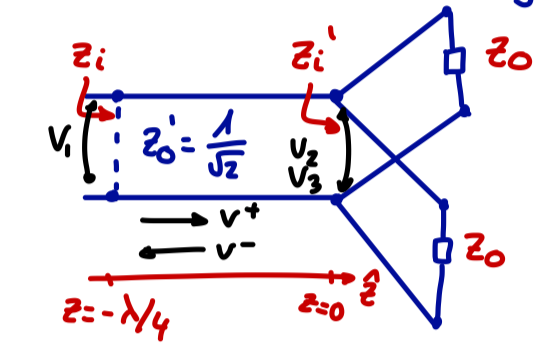
\includegraphics[width=7cm]{img/Divisor_en_lambda4_A_detalle.jpg}$$a=b$$
\end{center}

Para que el acceso 1 est\'e perfectamente adaptado, la impedancia a la entrada de la red ($z_i$) debe ser igual a la de la l\'inea ($z_0$). Empleando esta condici\'on para calcular la impedancia de la l\'inea que debenos emplear:
$$S_{11} = \cfrac{z_i - z_0}{z_i + z_0} = 0
\hspace{3mm}\rightarrow\hspace{3mm}
z_i = \cfrac{z'^2_0}{z'_i} = \cfrac{z'^2_0}{z_0 || z_0} = 1
\hspace{3mm}\rightarrow\hspace{3mm}
z'_0 = \cfrac{1}{\sqrt{2}}$$

Para calcular $S_{21}$ (que, por la simetr\'ia de nuestro divisor de potencia equivale a $S_{31}$, y por reciprocidad a $S_{12}$ y $S_{13}$), partimos de su definici\'on como factor de transmisi\'on en la red cuando los accesos est\'an acabados\footnote{De forma general, esto quiere decir que no hay onda entrante en el acceso 2 ($a_2 = 0 \rightarrow V_2 = V_2^-$). En este caso, adem\'as, encontramos que el factor de reflexi\'on en el acceso 1 ($S_{11}$) es 0, por lo que no hay onda saliente ah\'i ($b_1 = 0 \rightarrow V_1 = V_1^+$).}:
$$S_{21} = \cfrac{b_2}{a_1}\bigg|_{a_2 = a_3 = 0} = \cfrac{V_2^-}{V_1^+} = \cfrac{V_2}{V_1}$$

Puesto que los accesos 1 y 2 est\'an en los extremos de una l\'inea ($V(z) = V^+e^{-j\beta z} + V^-e^{j\beta z}$), podemos expresar sus tensiones de la forma:
$$\begin{array}{r@{}l@{=}l@{+}l@{=}r@{}r}
	V_2 &= V_{z=0} & V^+ e^{j0} & V^- e^{-j0} & V^+ +& V^-\\
	\\
	V_1 &= V_{z=\frac{\lambda}{4}} & V^+ e^{j\pi/2} & V^- e^{-j\pi/2} & jV^+ -& jV^- 
\end{array}$$

Relacionando las ondas progresiva y regresiva seg\'un el factor de reflexi\'on en $z = 0$:
$$\begin{array}{c}
	V^- = \rho V^+ \\
	\\
	\rho = \cfrac{z_i' - z_0'}{z_i' + z_0'} = \cfrac{1-\sqrt{2}}{1+\sqrt{2}}
\end{array}
\hspace{3mm}\rightarrow\hspace{3mm}
\cfrac{V_2}{V_1} = \cfrac{V^+ (1+\rho)}{jV^+(1-\rho)} = -\cfrac{j}{\sqrt{2}}$$


\paragraph{Divisores Resistivos}

Cuando abordamos el an\'alisis de divisores de potencia basados en elementos resistivos, hay que tener en cuenta que las p\'erdidas inherentes a este tipo de componentes nos impiden aplicar la condici\'on de unitariedad, por lo que nos vemos obligados a considerar s\'olo la pasividad y la reciprocidad.
\end{document}














































